Here are a few important questions that we might seek to address:
Linear model is a model of the form:
$$ p(y|\bm{x}, \bm{\theta}) = \mathcal{N}\left(
\bm{\beta}^{T}\bm{x},\sigma^{2}\right)$$.
Linear regression can be made to model non-linear reltationships by replacing
$\bm{x}$ with some non-linear function of the inputs $\phi$
$$ p(y|\bm{x}, \bm{\theta}) = \mathcal{N}\left(
\bm{\beta}^{T}\phi(\bm{x}),\sigma^{2}\right)$$.
\subsection{Simple linear regression}
In general simple linear regression is written as:\encV{$Y\approx
\beta_{0}+\beta_{1}X$}.\\We might read ``$\approx$'' as ``is 
approximately modeled as''

\paragraph{Estimating the Coefficients}
Let $\left\{ \left( x_{i},y_{i} \right) \right\}_{1\leq i\leq n}$
represent $n$ observations, our goal is to obtain coefficient estimates
$\widehat{\beta}_{0},\widehat{\beta}_{1}$ such that the linear model
fits the available data well, so that $y_{i}\approx\beta_{0}+\beta_{1}
x_{i}$ for $i\in\inter{1}{n}$, in other words we want an \emph{
intercept} $\beta_{0}$ and a \emph{slope} $\beta_{1}$\\For $i\in\inter{1
}{n}, e_{i}=y_{i}-\widehat{y}_{i}$ represents the $i^{th}$ \emph{
residual}\\
Then we define the \begin{center}\enc{$\text{RSS(\tR{Residual Sum of
Squares})}=\su{{i=1}}{n}e_{i}^{2}=\su{{i=1}}{n}\left( y_{i}- \widehat{
\beta_{0}}-\widehat{\beta_{1}}x_{i}\right)^{2}$}\end{center}.Using some calculus show 
that minimizers are \enc{$\begin{cases}\widehat{\beta_{1}}=\dfrac{\su{{
i=1}}{n}(x_{i}-\overline{x})(y_{i}-\overline{y})}{\su{{i=1}}{n}(x_{i}-
\overline{x})^{2}}\\\widehat{\beta}_{0}=\overline{y}-\widehat{\beta}_{1
}\overline{x}\end{cases}$}
\begin{figure}[H]
  \centering
  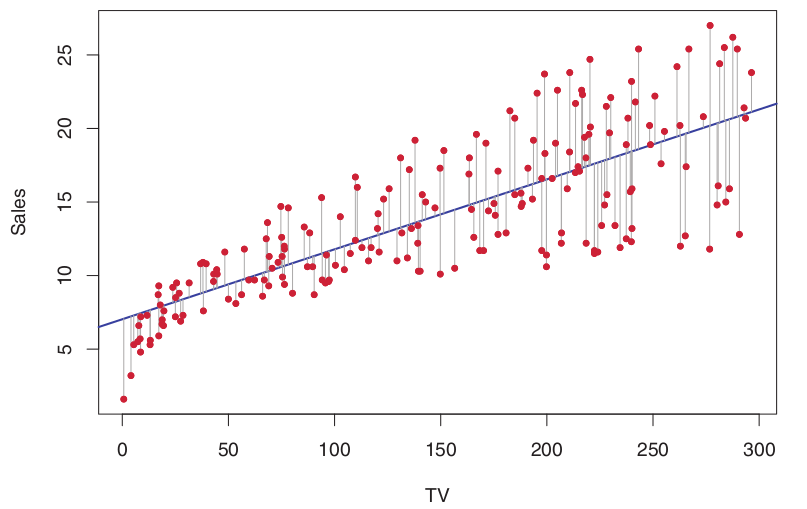
\includegraphics[width=.3\textwidth]{./chap/1chap/2sec/1images/1_leastSquares.png}
  \caption{The least squares fit for the regression of sales onto TV.}
  \label{fig:2.1}
\end{figure}
We can see on the following plots, that $\widehat{\beta}_{0},\widehat{\beta}_{1}$ minimize the RSS.
\begin{figure}[H]
  \centering
  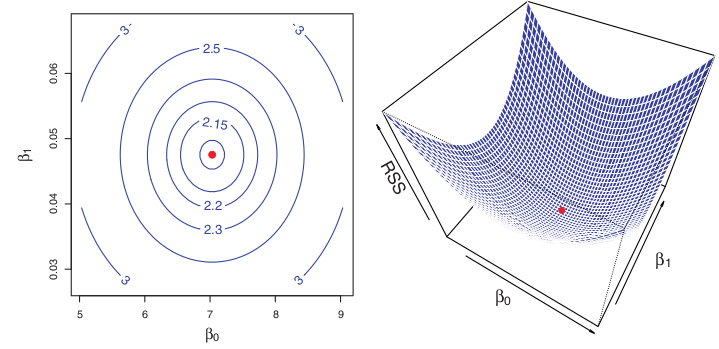
\includegraphics[width=.5\textwidth]{./chap/1chap/2sec/1images/2_leastSquaresCoefficients.png}
  \caption{Contour and 3-dimensionnal plots of the RSS on the 
Advertising data, using sales as the response and TV as the predictor}
  \label{fig:2.2}
\end{figure}

\paragraph{Assessing the Accuracy of the Coefficient Estimates}
When we assume that there is a relation between $X\text{ and }Y$ then
$Y=f\left( X \right)+\epsilon\begin{cases}f\text{ is a uknown function
 }\\\epsilon\text{ is a mean-zero random error term, is a catch-all for
what we miss with this simple model}\end{cases}$\\If $f$ is to be 
approximated by a linear function then we can write this relationship
as \encN{$Y=\beta_{0}+\beta_{1}X+\epsilon$}.\\This equation defines the
\emph{population regression line} which is the best approximation to
the true relationship between $X$ and $Y$.\\ We created $100$ random
$X_{s}$ and generated $100$ corresponding $Y_{s}$ from the model $Y=2+
3X+\epsilon$ where $\epsilon$ is generated from a normal distribution
with mean zero.
\begin{figure}[H]
  \centering
  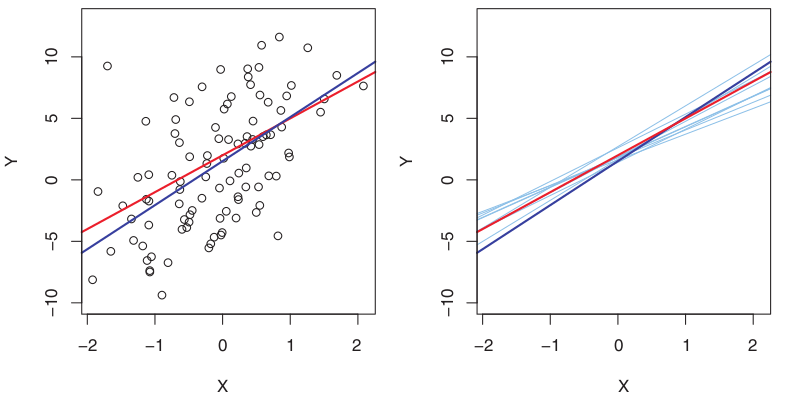
\includegraphics[width=\textwidth]{./chap/1chap/2sec/1images/3_leastSquaredErrorLineVsPopulationRegressionLine.png}
  \caption{The left-hand pannel:red line is the popuation regression
  line, and in blue line the least squares estimate for $f(X)$ bassed
  on the observed data, shown in black.\\The right-hand pannel: is the
  same graph that left-hand pannel but with 10 other least sqaures
  estimates with each a distinct training data set but from the same
  model}
  \label{fig:2.3}
\end{figure}
If we use the sample mean $
\widehat{\mu}$ to estimate $\mu$ this estimate is \emph{unbiased}, in
the sense that on average, we expect $\widehat{\mu}$ to equal $\mu$\\
We have etablished that the average $\widehat{\mu}$'s over many data
sets will be very close to $\mu$ but that a single estimate $\widehat{
\mu}$ may be a substantial underestimate or overestimate of $\mu$.
\tB{How far off will that single estimate of $\mu$ be? We generally 
answer to this question by computing the \emph{SE (Standard Error)} of
$\widehat{\mu}$ written as $SE(\widehat{\mu})$}:\begin{center}\enc{
$\V{\widehat{\mu}}=SE\left( \widehat{\mu} \right)^{2}=\dfrac{\sigma^{2}
}{n}$}\\$\sigma$ is the standard deviation of each of the realizations 
$y_{i}$ of $Y$.\end{center}
\begin{center}\enc{$
\begin{cases}SE\left(\widehat{\beta}_{0}\right)^{2}=\sigma^{2}\left[
\dfrac{1}{n}+\dfrac{\overline{x}^{2}}{\su{{i=1}}{n}\left(x_{i}-
\overline{x}\right)^{2}}\right]\\
SE\left(\widehat{\beta}_{1}\right)^{2}=
\dfrac{\sigma^{2}}{\su{{i=1}}{n}\left(x_{i}-\overline{x}
\right)^{2}}\end{cases}$}\\$\sigma^{2}=\V{\epsilon}$\end{center}\Moi{$SE\left(\widehat{\beta_{1}}
\right)$ is smaller when the $x_{i}$ are more spread out}For these
formulas we need to assume that the errors $\epsilon_{i}$ are
uncorrelated with $\sigma^{2}$. This is cleary not true but the formula
still turn out to be a good approximation.\\\sB{In general $\sigma$ is
unknown but can be estimated from the data, the estimate of $\sigma$ is
known as} \tR{\emph{Residual Standard Error}} \encB{$RSE=\sqrt{\dfrac{
RSS}{n-2}}$}.\\\Moi{Roughly speaking when $\sigma^{2}$ is estimated we
should write $\widehat{SE\left(\widehat{\beta_{1}}\right)}$}\\\\
Standard can be used to define \emph{confident interval}
\tR{For linear regression the $95\%$ confident intervals are} \begin{center}
\enc{$\begin{cases}\widehat{\beta_{0}}\pm 2\times SE\left(\widehat{
\beta_{0}}\right)\\\widehat{\beta_{1}}\pm 2\times SE\left(\widehat{
\beta_{1}}\right)\end{cases}$}\end{center}Standard error can be used
to perform hypothesis test, the most common test involves \emph{null
hypothesis} and \emph{alternative hypothesis}:\encB{$\begin{cases}
H_{0}:\beta_{1}=0\\H_{\alpha}:\beta_{1}\neq 0\end{cases}$}\\To test
null hypothesis we need to determine wehter $\widehat{\beta_{1}}$ is
sufficiently
far from zero that we can be confident that $\beta_{1}$ is non-null.\\
\emph{How far is far enough?} This depends on the $\widehat{\beta_{1}}$
accuracy then \\$\begin{cases}SE\left(\widehat{\beta_{1}}\right)\text{
is small, even relatively small values of }\widehat{\beta_{1}}\text{
can be a strong evidence that }\beta_{1}\neq 0\\SE\left(\widehat{
\beta_{1}}\right)\text{ is large then }\widehat{\beta_{1}}\text{ must 
be large in absolute value in order for us to reject }H_{0}\end{cases}$
\\In practice we compute a \emph{t-statistic} given by \begin{center}
\enc{$t=\dfrac{\widehat{\beta_{1}}-0}{SE\left(\widehat{\beta_{1}}
\right)}$}\\which measure the number of standard deviation that $
\widehat{\beta_{1}}$ is away from $0$.\end{center} \tB{If there is no
relationship between $X$ and $Y$ then we except that we will have a 
\emph{ t-distribution}}. It is a simple matter \tR{to observe the 
probability of observing any number equal to $|t|$ or larger in
absolute
value, \emph{assuming that }$\beta_{1}=0$} this probability is called
\tR{\emph{p-value}}.\\Roughly speaking a small \emph{p-value} indicates
that it is unlikely to observe such a substantial association between
the predictors and the response due to chance.\\\encN{Typical \emph{
p-value} cutoffs for rejecting $H_{0}$ is $5-1\%$}
\paragraph{Assessing the accuracy of the model}
Once we have rejected the null hypothesis in favor of the alternative
hypothesis it is natural to want to qualify to which the model fits the
data.
\subparagraph{Residual Standard Error} \tB{is an estimate of standard
deviation of $\epsilon$}, it means the average amount that the response
will deviate from the true regression line.
\subparagraph{$R^{2}$ statistic} it provides an alternative measure of
fit, and takes the form of a \emph{proportion} (the proportion of
variance explained). \tB{\emph{Total Sum of Squares}} \enc{$TSS=\su{{i=1}}{n
} \left(y_{i}-\overline{y}\right)^{2}$} represents the amount of 
variability
inherent to the response before the regression is performed, in 
contrast \emph{RSS measures the amount of variability that left
unexplained after performing regression}. \begin{center}\enc{$R^{2}=
	\dfrac{TSS-RSS}{TSS}$}\\Then $R^{2}$ measures the \emph{proportion of
variability in $Y$ that can be explained using $X$}\end{center}Recall
that \tR{correlation} defined as \begin{center}\enc{$\widehat{Cor(X,Y)}=
\dfrac{\su{ {i=1}}{n}\left(x_{i}-\overline{x}\right)\left(y_{i}-
\overline{y}\right)}{\sqrt{\su{ {i=1}}{n}\left(x_{i}-\overline{x}
\right)^{2}}\sqrt{\su{ {i=1}}{n}\left(y_{i}-\overline{y}\right)^{2}}}
$}\\$r=\widehat{Cor\left(X,Y\right)}$ is also a measure of the linear
relationship between $X$ and $Y$\end{center}\Moi{it can be shown that
in the simple regression setting $R^{2}=r^{2}$}

\subsection{Multiple linear regression}
\paragraph{Estimating the Regression Coefficients}
A common way to estimate the parameters of a statistical model is to compute
the MLE(Maximum Likelihood Estimation) defined as 
$$\hat{\bm{\theta}} \triangleq \displaystyle \argmax_{\theta} \log\left(
p(\mathcal{D}|\bm{\theta})\right)$$
\begin{align*}
    l(\bm{\theta}) &\triangleq \log\left(p(\mathcal{D}|\bm{\theta})\right)\\
                   &=\su{i=1}{n}\log\left(p(y_{i}|\bm{x_{i}}, \bm{\theta})\right)\\
                   &= \su{i=1}{n}\log\left(
                       \left[\dfrac{1}{2\pi\sigma^{2}}\right]^{\frac{1}{2}}
                       \exp\left(-\dfrac{1}{2\sigma^{2}}\left[y_{i} - \bm{\beta}^{T}
                       \bm{x_{i}}]\right]^{2}\right)\right)\\ 
                   &= \dfrac{1}{2\sigma^{2}}RSS(\bm{\beta}) +
                   \dfrac{n}{2}\log(2\pi\sigma^{2})
\end{align*}
Then the Residual Sum of Squares (RSS) is equal to $\su{i=1}{n}\left(
y_{i}-\beta^{T}x_{i}\right)^{2}$
Instead of maximizing the log-likelihood we can equivalently minimize the Negative Log Likelihood (NLL) 
\begin{center}
    $NLL(\beta) \triangleq l(\beta)$
\end{center}


Considering $\bm{X}$ the $N\times (p+1)$ matrix with each row an input
vector and $y$ be the $N-vector$ of outputs in the training set.
\begin{center}
	$RSS(\beta)=(y-\bm{X}\beta)^{T}(y-\bm{X}\beta)$
\end{center}
Differentiating with respect to $\beta$ we obtain:
$
\begin{cases}
	\dfrac{\partial RSS}{\partial\beta}=-2\bm{X}^{T}(y-\bm{X}\beta)\\
	\dfrac{\partial^{2} RSS}{\partial\beta\partial\beta^{T}}=2\bm{X}^{T}\bm{X}\\
\end{cases}
$\\
Assuming that $\bm{X}$ has full column rank, we set the first 
derivative to 0:\\ $\bm{X}^{T}(y-\bm{X}\beta)=0$ to obtain the unique
solution:

\begin{center}
	\encB{$\hat{\beta}=(\bm{X}^{T}\bm{X})^{-1}\bm{X}^{T}\bm{y}$}
\end{center}
\begin{figure}[H]
\centering
\begin{subfigure}{.5\textwidth}
  \centering
	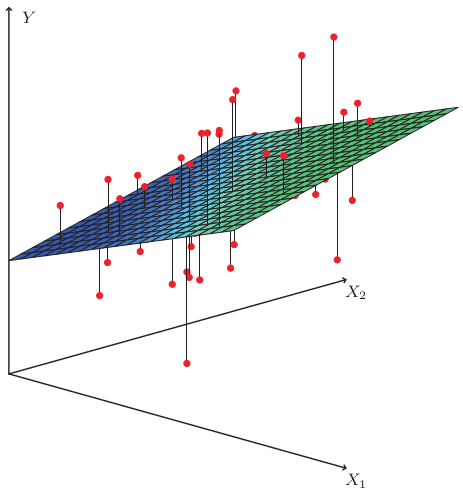
\includegraphics[width=.7\textwidth]{./chap/1chap/2sec/2images/1leastSquaresPlan.png}
  \caption{$n$ observations}
  \label{fig:2.1aLeastSquares}
\end{subfigure}%
\begin{subfigure}{.5\textwidth}
  \centering
	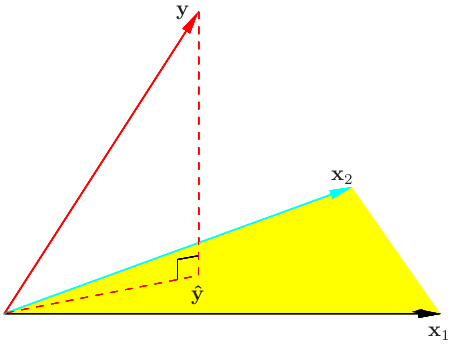
\includegraphics[width=\textwidth]{./chap/1chap/2sec/2images/11projection.png}
\caption{1 observation}
  \label{fig: 2.1bLeastSquares}
\end{subfigure}
  \caption{Least squares for a linear model with $2$ predictors of 
$p$-dimensions.}
\label{fig:test}
\end{figure}

\begin{align*}
\hat{\bm{y}} &=\bm{X}\hat{\beta}\\
	     &=\bm{X}\left(\bm{X}^{T}\bm{X}\right)^{-1}\bm{X}^{T}\bm{y}\\
	     &=\bm{H}\bm{y}
\end{align*}
$\bm{H}$ is called \tB{``hat'' matrix because it puts the hat on $\bm{y}$}.
\paragraph{Hat Matrix}
Residuals can also be expressed as a function of $\bm{H}$,
$\bm{\hat{e}} = \bm{y} - \bm{\hat{y}} = \bm{y} - \bm{Hy} = (\bm{I}-\bm{H})\bm{y}$.
It can be shown that \sB{$\bm{H}$ and $\bm{I}-\bm{H}$ are orthogonal projections}.\\
One can easily show that \tB{$\bm{H}\bm{H} = \bm{H}$} and $\left(\bm{I-H}\right)\left(\bm{I-H}\right)
= \bm{I-H}$

\subparagraph{Range and Kernel of the Hat Matrix}
$rank(\bm{X}) = rank(\bm{X}^{T}\bm{X}) = p^{*}$
\subparagraph{Residual and Fitted Values}
$\bm{H}(\bm{I}-\bm{H}) = \bm{H} -\bm{HH} = 0$, hence $\sP{\bm{\hat{y}}}{\bm{\hat{e}}} = 0$.
\tB{Therefore $\bm{\hat{y}}$ and $\bm{e}$ are orthogonal} in $\mathbb{R}^{n}$.
\subparagraph{Geometric interpretation}
The degrees of freedom associated with \tB{$\bm{\hat{y}}$ and $\bm{\hat{e}}$ can be seen to simply
be the dimensions of the respective vector subspace in which these 2 vectors have been projected}.\\
The vectors $\bm{y}, \bm{\hat{y}}$ and $\bm{\hat{e}}$ determine 3 points in $\mathbb{R}^{n}$ which
form a right-angled triangle, we can see the decomposition of total sum of squares into estimated
sum of squares and residual sum of squares as a special case of \emph{Pythagoras} theorem.
\subparagraph{Further information}
It might happen that the columns of \sB{$\bm{X}$ are not linearly independent, then
$\bm{X}^{T}\bm{X}$ is singular and the least squares coefficients $\hat{\beta}$ are not uniquely 
defined}.\\ 
Knowing that $\V{\bm{A}\bm{y}}=\bm{A}\V{\bm{y}}\bm{A}^{T}$:
\begin{center}
	\encB{$\V{\hat{\beta}}=\left(\bm{X}^{T}\bm{X}\right)^{-1}\sigma^{2}$}
\end{center}
a estimate of $\sigma^{2}$:$\hat{\sigma}^{2} = \dfrac{1}{N-p-1}\su{{i=1}}{N}(y_{i}-\hat{y}_{i})^{2}$ 
The $n-p-1$ rather than $n$ makes $\hat{\sigma}^{2}$ an unbiased
estimate.\\
$
\begin{cases}
\hat{\beta}\hookrightarrow\mathcal{N}\left(\beta, (\bm{X}^{T}\bm{X})^{-1}\sigma^{2}\right)\\
(n-p-1)\hat{\sigma}^{2}\hookrightarrow\sigma^{2}\chi_{n-p-1}^{2}
\end{cases}
$

\paragraph{Convexity}
Functions having a bowl shape with a unique minimum, more precisely:
$$\forall (\bm{\theta}, \bm{\theta'},\lambda) \in \mathcal{S}\times\mathcal{S}\times[0,1],
~ \lambda\bm{\theta} + (1-\lambda)\bm{\theta'} \in \mathcal{S} \Rightarrow \mathcal{S}
\text{ is \textbf{convex}}$$

\subsection{Assumption Checking}
\emph{Python Code}:
\begin{python}
import numpy as np
import pandas as pd
import statsmodels.api as sm
import statsmodels.stats.api as sms
from statsmodels.graphics.tsaplots import plot_acf
from statsmodels.sandbox.regression.predstd import wls_prediction_std
from statsmodels.tsa.ar_model import AutoReg
from statsmodels.tools.tools import add_constant

# Linear regression
y, X = df.iloc[:, 0], add_constant(df.iloc[:, 1:])
results_ols = sm.OLS(y, X).fit()
print(results.summary())

# Graphical representation of response
prstd, iv_l, iv_u = wls_prediction_std(results) # calculate standard deviation and confidence
interval for prediction
x = np.arange(y.shape[0])
fig, ax = plt.subplots()
ax.plot(x, y, 'o', label='Data')
ax.plot(x, results.fittedvalues, 'r--', label='Predicted')
ax.plot(x, iv_u, 'r--')
ax.plot(x, iv_l, 'r--')
ax.legend(loc='best')
plt.show()

# Checking of autoregressivity
mod_ar = AutoReg(results.resid, lags=3)
res_ar = mod_ar.fit()
print(res_ar.summary())

# Histogram, Q-Q plot, Correlogram ...
fig = res.plot_diagnostics(lags=30)
fig.tight_layout() # keeps space btw subplots
plt.show()
\end{python}

\emph{R code:}
\begin{rcode}[deletekeywords={2, df, model, resid, residuals}]
library(dplyr)
library(ggplot2)
library(lmtest) # testing linear regression

# Linear regression
model.ols <- lm(y ~ ., data=df)
summary(model.ols)

# Graphical diagnostic
resid <- model.ols$residuals # residuals
resid.std <- scale(model.ols$residuals) # standardized residuals

par(mfrow=c(2, 2))
plot(seq=(length(resid)), resid, xlab='No Obs.', ylab='Std Resid', main='Standardized Residuals')
hist(resid, xlab='Residuals', main='Histogram')
qqnorm(resid) # QQ plot
qline(resid) # Line QQ plot
pacf(resid, main='PACF for residuals')
\end{rcode}

\paragraph{Non-linearity of the Data}
\tB{Residual plots} are a useful graphical tool for identifying 
on-linearity.$\begin{cases}\text{simple regression: }plot(x_{i},e_{i})
	\text{ for the} i^{th} \text{observation}\\\text{multiple regression: }plot(
	\widehat{y}_{i},e_{i})\text{ for the} i^{th} \text{observation}\end{cases}$
The presence of a pattern may indicate a problem with some aspect of
the linear model.\\\tB{In non-linear setting, a simple approach might be
to apply non-linear transformation to predictors} (such as $\log\left(X
\right),\sqrt{X}\text{ and }X^{2}$) in the regression model.
\emph{Python code}
\begin{python}
import numpy as np
import matplotlib.pyplot as plt

res = results_ols.resid
yhat = results_ols.fittedvalues
poly = np.poly1d(np.polyfit(yhat, res, deg=3))
yhat_poly = np.linespace(yhat.min(), yhat.max(), yhat.shape[0])

fig, ax = plt.subplots()
ax.scatter(yhat, res)
ax.plot(yhat_poly, poly(yhat_poly), label='Polynomial estimation')
plt.xlabel('Fitted values')
plt.ylabel('Residuals')
plt.title('Residuals vs Fitted Values')
plt.show()
\end{python}

\emph{R code}
\begin{rcode}[deletekeywords={df, resid, lm, model, residuals, fitted, poly}]
library(ggplot2)

df.resid <- data_frame(res=lm.model$residuals, yhat=lm.model$fitted.values)
model.poly <- lm(res ~ poly(yhat,3), data=df.resid) # to evaluate the trend
df.resid$yhat.poly <- model.poly$fitted.values
df.resid %>% ggplot(aes(x=yhat))+
  geom_point(aes(y=res))+
  geom_line(aes(y=yhat.poly), color='blue')+
  geom_hline(aes(yintercept=0), linetype='dashed', color='red')+
  ggtitle('Non-linearity detection')
\end{rcode}

\paragraph{Correlation of error terms}
If the error are correlated we may have an unwarranted sense of 
confidence in our model.\\ To observe hypothetic correlation \tB{we can plot residuals
from our model as function of time.} If error are uncorrelated we 
should not observe any pattern.
\begin{figure}[H]
	\begin{center}
		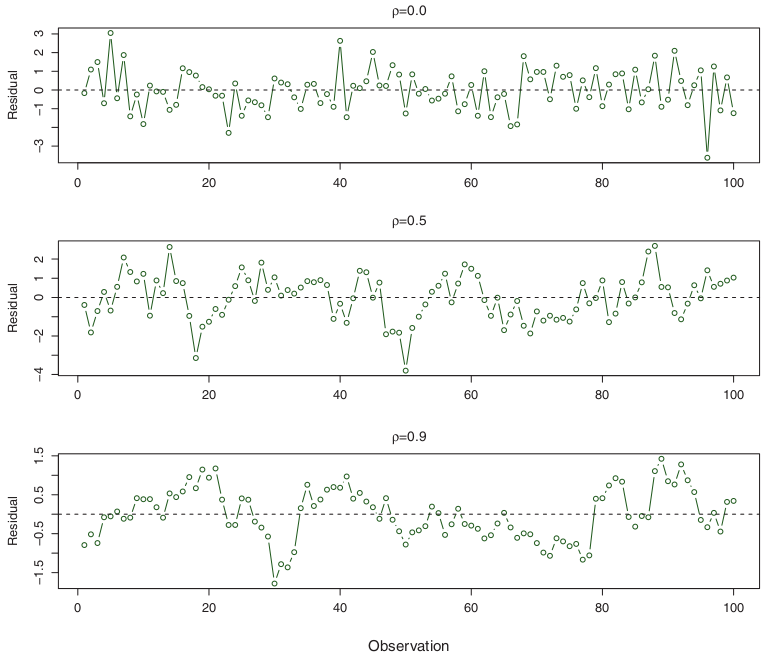
\includegraphics[width=.5\textwidth]{./chap/1chap/2sec/2images/2_7residualAsTimeSeries.png}
	\end{center}
	\caption{Residuals versus observation for given correlated
	coefficient, as we could plot for time series versus time.}
	\label{fig:fig2.7}
\end{figure}
\subparagraph{Definition Autocorrelation}
Disturbances are \emph{\textbf{autocorrelated}} when:
$$\forall (i,j)\in\inter{1}{n}^{2}\mathbb{C}ov\left(\epsilon_{i},\epsilon_{j}|\bm{X}\right)\neq0$$

$$ \text{Disturbances are \emph{autocorrelated} but are still assumed to be homoscedastic}
\Rightarrow $$
\begin{equation*}
	\Sigma=
	\begin{pmatrix}
		\sigma^{2} & \sigma_{12} & \cdots & \sigma_{1n}\\
		\sigma_{21} & \sigma^{2} & \cdots & \sigma_{2n}\\
		\vdots & \vdots & \ddots & \vdots\\
		\sigma_{n1} & \sigma_{n2} & \cdots & \sigma^{2}\\
	\end{pmatrix}
	= \sigma^{2}\Omega = \sigma^{2}
	\begin{pmatrix}
		1 & \omega_{12} & \cdots & \omega_{1n}\\
		\omega_{21} & 1 & \cdots & \omega_{2n}\\
		\vdots & \vdots & \ddots & \vdots\\
		\omega_{n1} & \omega_{n2} & \cdots & 1\\
	\end{pmatrix}
\end{equation*}
$\forall(i,j)\in\inter{1}{n}^{2},~\omega_{ij}=\dfrac{\sigma_{ij}}{\sigma^{2}}=corr(\epsilon_{i},
\epsilon_{j})$
\subparagraph{Autocorrelation Function (ACF)}
At each point $k$, representing lags, the function has the following value:
$$ \hat{r}_{k}=\dfrac{\su{{t=k+1}}{n}(x_{t-k}-\overline{x})(x_{t}-\overline{x})}{\su{{t=1}}{n}
(x_{t}-\overline{x})^{2}}
\begin{cases}
	k\in\inter{1}{n}\text{ representing the lag}\\
	x_{t}\text{ value of }x\text{ at row }t\\
	n\text{ number of observations in the series}
\end{cases}
$$

\emph{Python Code}
\begin{python}
import statsmodels.api as sm
from statsmodels.graphics.tsaplots import plot_acf

plot_acf(residuals, unbiased=True, zero=False,
    title='Residual autocorrelation')
plt.show()
\end{python}

\emph{R code}
\begin{rcode}[deletekeywords={df, resid}]
pacf(df.resid[, 'res'], main='Residual autocorrelation')
\end{rcode}

\subparagraph{Breusch-Godfrey test}
It is a \sB{test for autocorrelation in the errors in a regression model}.\\ 
Consider the linear regression :
$$ y_{t} = \beta_{0} + \beta_{1}X_{t,1} + \beta_{2}X_{t,2} + u_{t}
\begin{cases}
	u_{t} = \su{{k=1}}{p}\rho_{k}u_{t-k}+\epsilon_{t}\\
	\hat{u}_{t} = \alpha_{0} + \alpha_{1}X_{t,1} + \alpha_{2}X_{t,2} +
	\su{{k=1}}{p}\rho_{k}\hat{u}_{t-k} + \epsilon_{t}\text{ from the first OLS}
\end{cases}
$$
Then $R^{2}$ is computed and can be used for the distribution of the test statistic
$nR^{2}\hookrightarrow\chi_{p}^{2}$. When $H_{0}:\forall k\in\inter{1}{n}$ 
\emph{Python Code}
\begin{python}
import statsmodels.stats.api as sms
from sstatsmodels.tsa.ar_model import AutoReg

s_ar = pd.Series([AutoReg(result_ols.resid, lags=k) for k in range(1, 31)])
df_lag = pd.DataFrame({ # it will contain for each I.C. the optimal lag number
  'aic':[np.argmin(s.apply(lambda x: x.aic)) + 1],
  'hqic':[np.argmin(s.apply(lambda x: x.hqic)) + 1],
  'bic':[np.argmin(s.apply(lambda x: x.bic)) + 1]})
iter_l = [list(df_lag.iloc[0, :]).count(df_lag.iloc[0, j]) for j in range(df_lag.shape[1])] # occurence list
max_ind = max(range(len(iter_l)), key=iter_l.__getitem__) # index of the first value having the larger occurence number
lagOpt = df_lag.iloc[0, max_ind] #

test_BG = sms.acorr_breusch_godfrey(res=results_ols, nlags=lagOpt)
fscore_BG = test_BG[2]
fpvalue_BG = test_BG[3]
\end{python}

\emph{R code}
\begin{rcode}[deletekeywords={df, by, lm, model, max}]
library(VARS)
library(lmtest)

df.ar <- data_frame(res=lm.model$residuals) #
lagsel <- VARselect(df.ar$res, lag.max=30, type='const') # returning the optimal lag number
df.ar.count <- data_frame(lags=lagsel$selection, count=1) # count column contains 1's
df.ar.count %>% group_by(lags) %>%
  summarise(nbr=n()) %>%
  arrange(desc(nbr))
lagOpt <- df.ar.count$lags[1]
bgtest(lm.model, order=lagOpt) # Breusch-Godfrey test
\end{rcode}

The notation $AR(p)$ indicates an autoregressive model of order $p$. The $AR(p)$ model is defined
as $X_{t} = c + \su{{i=1}}{p}\phi_{i}X_{t-i} + \epsilon_{t}$ where $\phi_{k}$ are the parameters
of the model, $c$ is a constant and $\epsilon_{t}$ is a white noise.\\
The null hypothesis is that there is no serial correlation of any order up to $p$.
\begin{python}
glsar_model = sm.GLSAR(y, X, rho=1) # rho corresponds to the 
# order of the autoregressive covariance
glsar_results = glsar_model.iterative_fit(rtol=0.0001) # Relative tolerance between estimated 
# coefficients to stop the estimation
print(gls_results.summary())
\end{python}



\paragraph{Non-constant variance of error terms}
Hypothesis which is to consider the error terms have a constant variance
($\V{\epsilon_{i}}=\sigma^{2}$). Unfortunately is often the case that
variance of error terms is non-constant, then \tB{a solution might be to
transform response $Y$ using a concave function} such as $\sqrt{Y}\text{
or }\log\left(Y\right)$
\begin{figure}[H]
	\begin{center}
		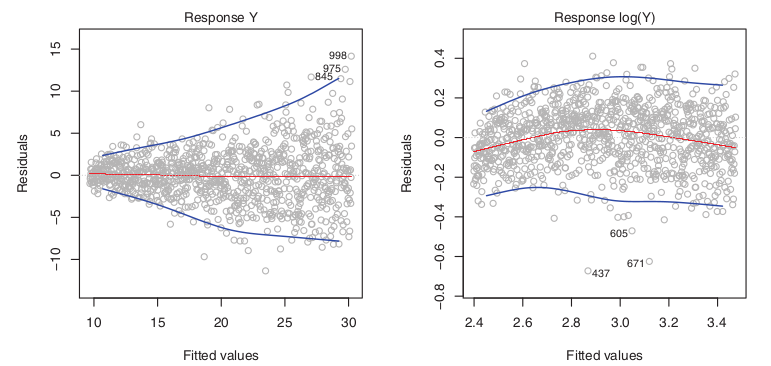
\includegraphics[width=\textwidth]{./chap/1chap/2sec/2images/2_8correctionOfNonConstantErrorTerms.png}
	\end{center}
	\caption{Residuals plots. In each plot the red line is a smooth
	fit to the residuals, intended to make it easier to identify
	a trend. The blue lines track the outer quantiles of the
	residuals and emphasis pattern. Left:The funnel shape indicates
	\emph{heteroscedasticity}. Right: The response has been log
	transformed, and there is now no evidence of heteroscedasticity
	.}
	\label{fig:fig2.8}
\end{figure}
To fix it: 
\begin{itemize}
	\item \tB{Check if important explanatory variables are missing in my model}
		and add them in.
	\item Switch to a \tB{GLM}, \tB{WSS}, or \tB{GLS} model
	\item \tB{A small amount of heteroscedasticity in the model's residual can be tolerated}
		if my model is otherwise performing well.
\end{itemize}
To diagnose there is \tB{Breush-Pagan test}:\\
Under the classical assumptions, OLS is the best linear unbiased estimator (BLUE), it is unbiased
and efficient. It remains unbiased under heteroscedasticity but efficiency is lost.\\
%The Breush-Pagan test is biased on models of type $\sigma_{i}^{2}=h(z_{i}'\gamma)$ for the 
%variances of the observations where $z_{i}=(1, z_{i2}, \cdots, z_{ip})$ explain the difference
%in the variances. $H_{0}:\forall j\in\inter{2}{p}\gamma_{j}=0$\\
The \emph{Method of Lagrange multipliers} \tB{is a strategy for finding the local maximal and
minima of a function subject to the condition that one or more equations} have to be satisfied
exactly by the chosen values of the variables.
The following Lagrange multiplier yields the  test statistic for the Breush-Pagan test:
$$ LM = \left(\dfrac{\partial l}{\partial\theta}\right)^{T}\left(-\E{\dfrac{\partial^{2}l}{\partial\theta\partial\theta'}}\right)^{-1}\left(\dfrac{\partial l}{\partial\theta}\right)$$
\begin{enumerate}
	\item Apply OLS: $\forall i\in\inter{1}{n} y_{i}=\beta X_{i} + \epsilon_{i}$
	\item Compute the regression residuals: $\hat{\epsilon}_{i}$, square them and divide by 
		the Maximum Likelihood Estimate of the error variance to obtain what Breusch and
		Pagan call $g_{i}$:\\
		$g_{i}=\dfrac{\hat{\epsilon}_{i}}{\su{{i=1}}{n}\frac{\hat{\epsilon}_{i}}{n}}$\\
		Estimate the auxiliary regression:
		$g_{i} = \gamma_{1} + \su{{j=2}}{p}\gamma_{j}z_{ij} +\eta_{i}$ where the $z$ terms
		will typically but not necessarily be the same as the original covariates $X$
	\item The LM test statistic is then half of the explained sum of squares from the 
		auxiliary regression: $LM = \dfrac{1}{2}\left(TSS-RSS\right)$
\end{enumerate}
%In GLM, $\bm{y}$ is assumed to be generated from a particular distribution in an exponential
%family (normal, binomial, Poisson, Gamma,\ldots) we have:
%$$ \E{\bm{y}}=\mu=g^{-1}\left(\beta\bm{X}\right)$$
%where $g$ is the link function.\\
%The GLM consists of 3 elements:
%\begin{enumerate}
%	\item An exponential family of probability distribution
%	\item A linear predictor $\eta=\beta\bm{X}$
%	\item A link function $g$ such that $\E{Y|X}=\mu=g^{-1}(\eta)$
%\end{enumerate}
%\begin{enumerate}
%	\item \textbf{Probability distribution}\\
%		Exponential family whose density functions:\\
%		$$f_{\bm{y}}(\bm{y}|\theta,\tau)=h(\bm{y},\tau)\exp\left(\dfrac{b(\theta)^{T}
%		\bm{T}(\bm{y})-\bm{A}(\theta)}{d(\tau)} \right)$$
%		$\theta$ is related to the mean of the distribution, $b$ is the identity function
%		The \emph{dispersion parameter} $\tau$, typically is known and is usually related
%		to the variance of the distribution.
%		$\begin{cases}
%			\mu = \E{\bm{y}} = \nabla \bm{A}(\theta)\\
%			\V{\bm{y}} = \nabla^{2}\bm{A}(\theta)d(\tau)
%		\end{cases}
%			$
%	\item \textbf{Linear predictor}\\
%		It is the quantity which incorporates the information about the independent 
%		variables into the model. 
%		$$\eta=\beta\bm{X}$$
%	\item \textbf{Link function}\\
%		It provides the relationship between the linear predictor and the mean of the 
%		distribution function. 
%		\begin{figure}[H]
%			\begin{center}
%				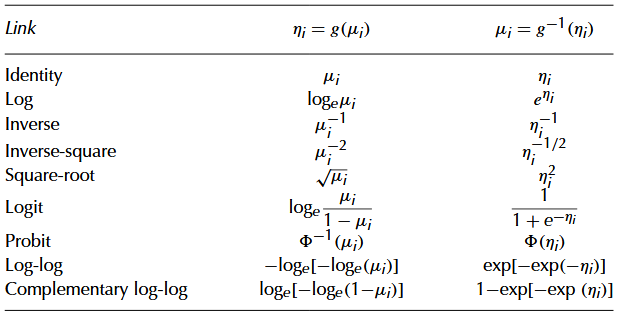
\includegraphics[width=.8\textwidth]{./chap/1chap/2sec/3images/5_glm.PNG}
%			\end{center}
%			\caption{$\mu_{i}$ is the expected value of the response; $\eta_{i}$ is
%			the linear predictor and $\Phi$ the cumulative distribution function of 
%			standard-normal distribution.}
%			\label{fig:5_glm}
%		\end{figure}
%\end{enumerate}

%\begin{lstlisting}
%# for example if data seem to have a gamma distribution:
%gamma_model = sm.GLM(y, X, family=sm.families.Gamma())
%gamma_results = gamma_model.fit()
%\end{lstlisting}


\paragraph{Generalized Linear Regression Model and Heteroscedasticity}
\subparagraph{Generalized Linear Regression Model }
$$
\begin{cases}
	\bm{y} = \bm{X}\bm{\beta} + \bm{\epsilon}\\
	\E{\bm{\epsilon}|\bm{X}} = \bm{0}_{n\times 1}\\
	\V{\epsilon|\bm{X}} = \bm{\Sigma} = \sigma^{2}\bm{\Omega}
\end{cases}
$$
where $\bm{X}$ is a matrix of fixed or random regressors, $\beta\in\mathbb{R}^{k}$, $\Sigma,
\Omega$ are symmetric positive definite matrices. 

\begin{equation*}
	\Sigma=
	\begin{pmatrix}
		\sigma_{1}^{2} & \sigma_{12} & \cdots & \sigma_{1n}\\
		\sigma_{21} & \sigma_{2}^{2} & \cdots & \sigma_{2n}\\
		\vdots & \vdots & \ddots & \vdots\\
		\sigma_{n1} & \sigma_{n2} & \cdots & \sigma_{n}^{2}\\
	\end{pmatrix}
= \sigma^{2}
	\begin{pmatrix}
		\omega_{1}^{2} & \omega_{12} & \cdots & \omega_{1n}\\
		\omega_{21} & \omega_{2}^{2} & \cdots & \omega_{2n}\\
		\vdots & \vdots & \ddots & \vdots\\
		\omega_{n1} & \omega_{n2} & \cdots & \omega_{n}^{2}\\
	\end{pmatrix}
\end{equation*}
and $\forall(i,j)\in\inter{1}{n}^{2},~\omega_{ij}=\dfrac{\sigma_{ij}}{\sigma^{2}}$
\subparagraph{Definition Heteroscedasticity}
Disturbances are \emph{\textbf{heteroscedastic}} when they have different (conditional) 
variances:
$$\forall (i,j)\in\inter{1}{n}^{2},~i\neq j\Rightarrow \V{\epsilon_{i}|
\bm{X}_{i\bullet}}\neq\V{\epsilon_{j}|\bm{X}_{j\bullet}}$$

$$ \text{Disturbances are \emph{heteroscedastic} but are still assumed to be uncorrelated across
observations}\Rightarrow $$
\begin{center}
\begin{equation*}
	\Sigma=
	\begin{pmatrix}
		\sigma_{1}^{2} & 0 & \cdots & 0\\
		0 & \sigma_{2}^{2} & \cdots & 0\\
		\vdots & \vdots & \ddots & \vdots\\
		0 & 0 & \cdots & \sigma_{n}^{2}\\
	\end{pmatrix}
	= \sigma^{2}\bm{\Omega}=\sigma^{2}
	\begin{pmatrix}
		\omega_{1}^{2} & 0 & \cdots & 0\\
		0 & \omega_{2}^{2} & \cdots & 0\\
		\vdots & \vdots & \ddots & \vdots\\
		0 & 0 & \cdots & \omega_{n}^{2}\\
	\end{pmatrix}
\end{equation*}
\end{center}



%\paragraph{Inefficency of the OLS}
%We start from the \emph{Generalized Linear Regression} model and here $\beta=\hat{\beta}_{OLS}
%\left( \bm{X}^{T}\bm{X} \right)^{-1}\bm{X}^{T}\bm{y} $. The regressors are exogenous in the sense
%that : $\E{\epsilon|\bm{X}}=\bm{0}_{N\times 1}$.
%OLS estimator is \textbf{\emph{unbiased}} $\Rightarrow \E{\hat{\beta}_{OLS}}=\beta_{0}$
%where $\beta_{0}$ denotes the true value of the parameters.
%Heteroscedasticity and/or Autocorrelation do not induce a bias for the OLS estimator.\\
%
%In GLR model, under exogeneity the OLS estimator has a conditional covariance matrix given by
%$$ \V{\hat{\beta}_{OLS}|\bm{X}}=\sigma_{0}^{2}\left(\bm{X}^{T}\bm{X}\right)^{-1}\bm{X}^{T}\Omega
%\bm{X}\left(\bm{X}^{T}\bm{X}\right)^{-1}$$
%Proof:
%\begin{align*}
%\begin{split}
%\hat{\beta}_{OLS} &= \left(\bm{X}^{T}\bm{X}\right)^{-1}\bm{X}^{T}\bm{y}\\
%&= \left(\bm{X}^{T}\bm{X}\right)^{-1}\bm{X}^{T}(\bm{X}\beta_{0}+\bm{\epsilon})\\
%&= \beta_{0} + \left(\bm{X}^{T}\bm{X}\right)^{-1}\bm{X}^{T}\bm{\epsilon}
%\end{split}
%\\\\
%\begin{split}
%\V{\hat{\beta}_{OLS}|\bm{X}} &= \V{\beta_{0} +
%\left(\bm{X}^{T}\bm{X}\right)^{-1}\bm{X}^{T}\bm{\epsilon}}\\
%&= \V{\left(\bm{X}^{T}\bm{X}\right)^{-1}\bm{X}^{T}\bm{\epsilon}}\\
%&= \E{\left(\bm{X}^{T}\bm{X}\right)^{-1}\bm{X}^{T}\bm{\epsilon}
%\left(\left(\bm{X}^{T}\bm{X}\right)^{-1}\bm{X}^{T}\bm{\epsilon}\right)^{T}|\bm{X}}
%\\
%&= \E{\left(\bm{X}^{T}\bm{X}\right)^{-1}\bm{X}^{T}\bm{\epsilon}\epsilon^{T}\bm{X}
%\left(\bm{X}^{T}\bm{X}\right)^{-1}|\bm{X}}\\
%&= \left(\bm{X}^{T}\bm{X}\right)^{-1}\bm{X}^{T}\E{\bm{\epsilon}\epsilon^{T}|\bm{X}
%}\bm{X}\left(\bm{X}^{T}\bm{X}\right)^{-1}\\
%&= \sigma_{0}^{2}\left(\bm{X}^{T}\bm{X}\right)^{-1}\bm{X}^{T}\bm{\Omega}\bm{X}
%\left(\bm{X}^{T}\bm{X}\right)^{-1}
%\end{split}
%\end{align*}
%
%Under exogeneity and normality, the OLS estimator obtained in the generalized linear regression
%model has an (exact) \emph{normal conditional distribution} :
%$$ \hat{\beta}_{OLS}|\bm{X}\hookrightarrow \mathcal{N}\left(\beta_{0},\sigma^{2}\left(\bm{X}^{T}
%\bm{X}\right)^{-1}\right)\bm{X}^{T}\bm{\Sigma}\bm{X}\left(\bm{X}^{T}\bm{X}^{-1}\right)$$
%
%Because the variance of the OLS estimator is not $\sigma^{2}\left(\bm{X}^{T}\bm{X}\right)^{-1}$
%statistical inference (\emph{non-robust inference}) based on $\hat{\sigma}^{2}\left(\bm{X}^{T}
%\bm{X}\right)^{-1}$ may be \emph{misleading}.\\
%The question is to know how to estimate $\V{\hat{\bm{\beta}_{OLS}}}$ in context of the linear
%generalized regression model in order to make \emph{robust inference}.
%In the GLR model under some regularity conditions:
%\begin{itemize}
%	\item  OLS is \emph{unbiased}
%	\item  OLS is (weakly) \emph{consistent}
%	\item  OLS is \emph{asymptotically normally distributed}
%\end{itemize}
%But the inference based on the estimator $\sigma^{2}\left(\bm{X}^{T}\bm{X}\right)^{-1}$ is 
%\emph{misleading}, OLS is \emph{inefficient} $\V{\hat{\bm{\beta}_{OLS}}}-I_{N}^{-1}(\bm{\beta}_{0}
%)$ is a positive definite matrix.
\paragraph{Weighted Least Squares (WLS)}
Weighted Least Squares is a generalization of ordinary least squares and linear regression in
which the errors covariance matrix is allowed to be different from an identity matrix. \sB{It is a
special case of Generalized Least Squares in which the covariance matrix is diagonal.}
The standard model assumes that $\forall i\in\inter{1}{n}\V{\epsilon_{i}}=\sigma^{2}$ whereas in
WLS we suppose $\exists\prth{\omega}{i}{n},~\forall i\in\inter{1}{n}\V{\epsilon_{i}}=
\dfrac{\sigma^{2}}{\omega_{i}}$ 
$$RSS(\beta)=\left(\bm{Y}-\bm{X}\beta\right)^{T}\bm{\Omega}\left(\bm{Y}-\bm{X}\beta\right)$$
Then $\dfrac{\partial RSS(\beta)}{\partial\beta}=0\Rightarrow \beta=
\left(\bm{X}^{T}\bm{\Omega}\bm{X}\right)^{-1}\bm{X}^{T}\bm{\Omega}\bm{Y}$

In general suppose we have the linear model: 
$\bm{Y} = \bm{X}\beta + \epsilon$ where $\V{\epsilon}=\bm{\Omega}^{-1}\sigma^{2}$, then we have
$\V{\bm{\Omega}^{\frac{1}{2}}\epsilon}=\sigma^{2}\bm{I}_{n}$\\
Hence we consider the transformation:
$
\begin{cases}
	\bm{Y}'=\bm{\Omega}^{\frac{1}{2}}\bm{Y}\\
	\bm{X}'= \bm{\Omega}^{\frac{1}{2}}\bm{X}\\
	\epsilon' = \bm{\Omega}^{\frac{1}{2}}\epsilon
\end{cases}
$\\
This give us $\bm{Y}=\bm{X}'\beta+\epsilon'$:
\begin{align*}
	\hat{\beta} &= \left( (\bm{X}')^{T}\bm{X}'\right)^{-1}(\bm{X}')^{T}\bm{Y}'\\
	&= \left(\bm{X}^{T}\bm{\Omega}\bm{X}\right)^{-1}\bm{X}^{T}\bm{W}\bm{Y}
\end{align*}

Advantages:
\begin{itemize}
	\item In WLS the interpretation of coefficient remains the same as OLS
	\item In WLS we generally include an intercept which means that the \emph{F-test} and 
		$R^{2}$ are interpreted as usual. 
	\item WLS gives us an easy way to remove one observation from a model by setting it 
		weight equal to 0
	\item  We can downweight outlier or leverage points to reduce their impact on the overall
		model.
\end{itemize}

The Weights
\begin{itemize}
	\item We may have a probabilistic model for $\mathbb{V}\left(\bm{Y}|\bm{X}=x_{i}\right)$
		in which case we would use this model to find the $\omega_{i}$
	\item Another common case is where each observation is not a single measure but an 
		average of $n_{i}$ actual measures and the original measures each have variance
		$\sigma^{2}$
	\item We would use WLS with weights $\omega_{i}=n_{i}$
\end{itemize}

\begin{lstlisting}
model_wls = sm.WLS(y, X, weights=1./(w**2))
result_wls = mod_wls.fit()
print(result_wls.summary())
\end{lstlisting}

\paragraph{Generalized Least Squares (GLS)}
Consider the generalized linear regression model with:
$$ \V{\bm{\epsilon}|\bm{X}} = \bm{\Sigma}=\sigma^{2}\bm{\Omega}$$
We will distinguish 2 cases:
\begin{enumerate}
	\item $\bm{\Sigma}$ is \emph{known}
	\item $\bm{\Sigma}$ is \emph{\textbf{un}known}
\end{enumerate}
\subparagraph{Known covariance matrix}
The Generalized Least Squares (GLS) estimator of $\bm{\beta}$ is defined as to be:
\tB{$$ \hat{\bm{\beta}}_{GLS} = \left(\bm{X}^{T}\Omega^{-1}\bm{X}\right)^{-1}\bm{X}^{T}\Omega\bm{y}$$}
Under the exogeneity assumption the estimator $\hat{\bm{\beta}_{GLS}}$ is \emph{unbiased}:
$\E{\hat{\bm{\beta}}_{GLS}}=\bm{\beta}_{0}$ where $\bm{\beta}_{0}$ denotes the true value of the
parameters.\\

Under suitable regularity conditions, in a parametric generalized linear regression model,
the GLS estimator $\hat{\bm{\beta}}_{GLS}$ is efficient! $\V{\hat{\bm{\beta}}_{GLS}}=I_{N}^{-1}
\left(\bm{\beta}_{0}\right)$, where $I_{N}^{-1}\left(\bm{\beta}_{0}\right)$ denotes the FDCR or 
Cramer-Rao bound.
\subparagraph{Unknown covariance matrix}
\sB{We assume that the conditional variance matrix of the disturbances can be expressed as a function
of a small set of parameters $\alpha$:}
$$ \V{\bm{\epsilon}|\bm{X}}=\sigma^{2}\bm{\Omega}(\alpha)$$
Consider a consistent estimator $\hat{\alpha}$ of $\alpha$ then the Feasible Least Generalized
Squares (FGLS) estimator of $\bm{\beta}$ is defined as to be:
\tB{$$ \hat{\bm{\beta}}_{FGLS} = \left(\bm{X}^{T}\hat{\bm{\Omega}}^{-1}\bm{X}\right)^{-1}
\bm{X}^{T}\hat{\bm{\Omega}}\bm{y}$$}
where \tB{$\hat{\bm{\Omega}}=\bm{\Omega}(\hat{\alpha})$ is a consistent estimator of 
$\bm{\Omega}(\alpha)$.}\\
An asymptotically efficient FGLS estimator does not require that we have an efficient estimator
of $\alpha$; only a consistent one is required to achieve full efficiency for the FLGS estimator.

\paragraph{Heteroscedasticity}
\begin{figure}[H]
	\begin{center}
		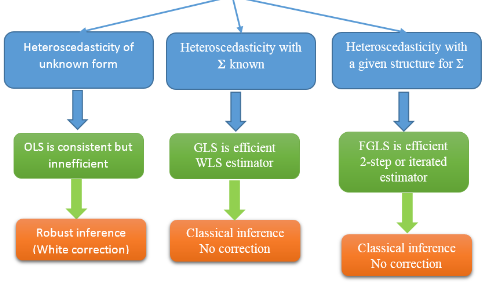
\includegraphics[width=\textwidth]{./chap/1chap/2sec/3images/6_heteroscedasticity.PNG}
	\end{center}
	\caption{Procedure to deal with heteroscedasticity}
	\label{fig:6_heteroscedasticity}
\end{figure}
\begin{enumerate}
	\item \textbf{\emph{Heteroscedasticity of unknown form}}\\
		 The conventionally estimated covariance matrix for the least squares estimator
		 $\sigma^{2}\left(\bm{X}^{T}\bm{X}\right)^{-1}$ is inappropriate, the appropriate
		 matrix is \\
		 $\sigma^{2}\left(\bm{X}^{T}\bm{X}\right)^{-1}\left(\bm{X}^{T}\Sigma
		 \bm{X}\right)^{-1}\left(\bm{X}^{T}\bm{X}\right)^{-1}$. It is unlikely that these 2 would coincide, so the usual estimators of the standard errors are 
		 likely to be erroneous. The inference (test-statistic) based $\sigma^{2}\left(
		 \bm{X}^{T}\bm{X}\right)^{-1}$\\
		 The \tB{\emph{White consistent} estimator of the \emph{asymptotic
		 covariance} matrix of the OLS estimator $\hat{\bm{\beta}}_{OLS}$} in the
		 generalized linear regression model is defined to be:
		 \tB{$\mathbb{V}_{asy}\left(\hat{\bm{\beta}}_{OLS}\right)=N\left(\bm{X}^{T}\bm{X}
		 \right)^{-1}\bm{S}_{0}\left(\bm{X}^{T}\bm{X}\right)^{-1}$}, with $\bm{S}_{0}=
		 \dfrac{1}{N}\su{{i=1}}{N}\hat{\epsilon}_{i}^{2}\sP{\bm{X}_{i\bullet}^{T}}{\bm{X}_{i\bullet}}$\\
\begin{python}
y, X = df.iloc[:, 0], df.iloc[:, 1:]
model_ols = sm.OLS(y, X)
result_ols_white = model_ols.fit(cov_type='HC0') # Applying White correction
print(result_ols_white.summary())
\end{python}

	\item \textbf{\emph{Heteroscedasticity with known $\Sigma$}}\\
		We assume that the disturbances are heteroscedastic with $\V{\bm{\epsilon}|
		\bm{X}}=\bm{\Sigma}=\sigma^{2}\bm{\Omega}$ with :
\begin{center}
\begin{equation*}
	\Sigma=
	\begin{pmatrix}
		\sigma_{1}^{2} & 0 & \cdots & 0\\
		0 & \sigma_{2}^{2} & \cdots & 0\\
		\vdots & \vdots & \ddots & \vdots\\
		0 & 0 & \cdots & \sigma_{n}^{2}\\
	\end{pmatrix}
	= \sigma^{2}\bm{\Omega}=\sigma^{2}
	\begin{pmatrix}
		\omega_{1} & 0 & \cdots & 0\\
		0 & \omega_{2} & \cdots & 0\\
		\vdots & \vdots & \ddots & \vdots\\
		0 & 0 & \cdots & \omega_{n}\\
	\end{pmatrix}
\end{equation*}
\end{center}
In presence of heteroscedasticity, the Generalized Least Squares (GLS) estimator of $\beta$ is 
defined as to:
\tB{$\hat{\bm{\beta}}_{GLS} = \left(\su{{i=1}}{n}\dfrac{x_{i}x_{i}^{T}}{\omega_{i}}\right)^{-1}
\su{{i=1}}{n}\dfrac{x_{i}y_{i}}{\omega_{i}}$}\\
In presence of heteroscedasticity, the GLS estimator is a particular case of the WLS estimator:
\tB{$\hat{\bm{\beta}}_{WLS} = \left(\su{{i=1}}{n}\delta_{i}x_{i}x_{i}^{T}\right)^{-1}
\su{{i=1}}{n}\delta_{i}x_{i}y_{i}$} where $\delta_{i}$ is an arbitrary weight.\\
For $\delta_{i}=\frac{1}{\omega_{i}}$ we have $\hat{\bm{\beta}}_{WLS}=\hat{\bm{\beta}}_{GLS}$\\
The WLS estimator is consistent regardless of the weights used, as long as the weights are 
uncorrelated with the disturbances. In general, we consider a weight which is proportional to
one explicative variable the income in the last example: 
$$ \sigma_{i}^{2} = \sigma^{2}x_{ik}^{2} \Leftrightarrow \delta_{i}=\dfrac{1}{x_{ik}^{2}}$$
\begin{python}
# Assuming y = y_true + sig * w * e
model_wls = sm.WLS(y, X, weights=1/w**2)
results_wls = model_wls.fit()
print(results_wls.summary())
\end{python}

	\item \textbf{\emph{Heteroscedasticity for a given structure}}\\
\begin{center}
\begin{equation*}
	\Sigma(\bm{\alpha})=
	\begin{pmatrix}
		\sigma_{1}^{2}(\bm{\alpha}) & 0 & \cdots & 0\\
		0 & \sigma_{2}^{2}(\bm{\alpha}) & \cdots & 0\\
		\vdots & \vdots & \ddots & \vdots\\
		0 & 0 & \cdots & \sigma_{n}^{2}(\bm{\alpha})\\
	\end{pmatrix}
	= \sigma^{2}\bm{\Omega}(\bm{\alpha})=\sigma^{2}
	\begin{pmatrix}
		\omega_{1}(\bm{\alpha}) & 0 & \cdots & 0\\
		0 & \omega_{2}(\bm{\alpha}) & \cdots & 0\\
		\vdots & \vdots & \ddots & \vdots\\
		0 & 0 & \cdots & \omega_{n}(\bm{\alpha})\\
	\end{pmatrix}
\end{equation*}
\end{center}
		We assume that the disturbances are heteroscedastic with :
		$\V{\bm{\epsilon}|\bm{X}}=\bm{\Sigma}(\alpha)=\sigma^{2}\bm{\Omega}(\bm{\alpha})(\bm{\alpha})$
		where $\bm{\alpha}$ denotes a set of parameters.\\
		Examples:\\
		We assume that $\mathbb{V}(\epsilon_{i}|\bm{X})=\sigma^{2}_{i}(\bm{\alpha})=
		\sigma^{2}\left(\bm{z}_{i}^{T}\bm{\alpha}\right)$ where $\bm{\alpha}=(\alpha_{1},
		\cdots, \alpha_{H})^{T}$ is a $H\times 1$ vector of parameters and $\bm{z}_{i}$
		is a $H\times 1$ of explicative variables (not necessarily the same as in $x_{i}$)
		\\ If we assume for instance that :
		$\V{\epsilon_{i}|\bm{X}}=\sigma_{i}^{2}(\bm{\alpha})=\exp(\bm{z}_{i}^{T}\bm{
		\alpha})$ where $\bm{z}_{i}$ is a vector of H variables, a way to estimate
		$\alpha$ consists in considering the model: $ln(\hat{\epsilon}_{i}^{2})=
		\bm{z}_{i}^{T}\bm{\alpha} + v_{i}$ and to estimate $\alpha$ by OLS. Given 
		$\hat{\alpha}$ we have a consistent estimator for $\sigma_{i}^{2}$, 
		$\sigma_{i}^{2} = \exp(\bm{z}_{i}^{T}\hat{\bm{\alpha}})\rightarrow\sigma_{i}^{2}(
		\bm{\alpha})$\\
		Consider the generalized linear regression model:\\
		$y_{i} = \beta_{0} + \beta_{1}\times age_{i} + \beta_{2}\times ownrent + \beta_{3}
		\times income_{i} + \beta_{4}\times income_{i}^{2}$\\ where the heteroscedasticity
		satisfies Harvey's specification:\\
		$\V{\epsilon_{i}|\bm{X}}=\sigma_{i}^{2}=\exp(\alpha_{0}+\alpha_{1}\times 
		income_{i})$\\
		A way to get the estimates of the parameters $\alpha_{1}$ and $\alpha_{2}$ is to
		consider the regression: $ln\left(\hat{\epsilon}_{i}^{2}\right)=\alpha_{0}+
		\alpha_{1}\times income_{i} + \eta_{i}$, with 
		$\eta\hookrightarrow\mathcal{N}(0,1)$
\begin{python}
beta = sm.OLS(y, X).fit().params # containing beta_0, ..., beta_4
diff = np.ones(beta.shape[0]) # array having as same 1's as beta length  

while max(diff) > 0.001:
    res = y - X.dot(beta)
    W = sm.add_constant(X.loc[:, 'Income']) 
    alpha = sm.OLS(np.log(residuals_ols**2), W).fit().params
    sigma = np.exp(W.dot(alpha)) # Harvey's specification
    beta_fgls = sm.GLS(y, X, sigma=sigma).fit().params
    diff = beta_fgls-beta
    beta = beta_fgls
\end{python}
	
		Estimate the parameters $\bm{\beta}$ by OLS. Compute the residuals 
		$\hat{\epsilon}_{i} = y_{i}-x_{i}^{T}\hat{\bm{\beta}}_{OLS}$ and estimate the 
		parameters $\alpha$ according to the appropriate model. Compute the estimated 
		variance $\sigma_{i}^{2}(\bm{\alpha})$ and compute the Feasible Generalized Least
		Squares (FGLS):
		\tB{$$ \hat{\bm{\beta}}_{FGLS}^{(1)}=\left(\su{{i=1}}{N}\dfrac{x_{i}x_{i}^{T}}{
		\sigma_{i}^{2}(\hat{\bm{\alpha}})}\right)^{-1}\su{{i=1}}{N}\dfrac{x_{i}y_{i}}{
		\sigma_{i}^{2}(\hat{\bm{\alpha}})}$$}
		Compute the residuals $\hat{\epsilon}_{i}=y_{i}-x_{i}^{T}\hat{\bm{
		\beta}}_{FGLS}^{(1)}$ and estimate the parameters $\bm{\alpha}$ according to the
		appropriate model. Compute the FGLS $\hat{\bm{\beta}}_{FGLS}^{(2)}$ and so on 
		$\cdots$. The procedure stop when:\\
		$\sup\limits_{j\in\inter{1}{K}}\left|\hat{\bm{\beta}}_{j,FGLS}^{(i)}-
		\hat{\bm{\beta}}_{j,FGLS}^{(i-1)}\right|<\text{ threshold (ex: 0.001)}$\\
		\sB{Avoiding this method when sample size is small.}
		
\end{enumerate}

The \textbf{White test for heteroscedasticity} is based on: 
$\begin{cases}
	H_{0}:\forall\inter{1}{N},~\sigma_{i}^{2}=\sigma^{2}\\
	H_{a}:\exists(i,j)\in\inter{1}{N}^{2},~\sigma_{i}^{2}\neq\sigma_{j}
\end{cases}
$
Procedure:
\begin{itemize}
	\item[\textit{Step 1}:] Estimation of the model using the OLS estimator of $\bm{\beta}$
	\item[\textit{Step 2}:] Determine the residual $\hat{\epsilon}_{i}=y_{i}-\bm{x}_{i}^{T}
		\hat{\bm{\beta}}_{OLS}$
	\item[\textit{Step 3}:] Regress $\hat{\bm{\epsilon}}_{i}^{2}$ on a constant and all unique
		columns vectors contained in $\bm{X}$ and all the squares and cross-products of
		the column vectors in $\bm{X}$.

	\item[\textit{Step 4}:] Determine the coefficient of determination, $R^{2}$, of the previous regression.
\end{itemize}
Under the null, the White test statistic $N\times R^{2}\rightarrow\chi^{2}(m-1)$ where $m$ is
the number of explanatory variables in the regression of $\hat{\epsilon}_{i}$.\\
The critical region of size $\alpha$ is:
$$ W = \left\{y:N\times R^{2}>\bm{\chi_{1-\alpha}}^{2}\right\}$$ where $\chi_{1-\alpha}^{2}$
denotes the $1-\alpha$ critical value of the $\chi^{2}(m-1)$ distribution.

\begin{python}
test_white = sms.het_white(residuals, X)
fvalue, fpvalue = test_white.fvalue, test_white.f_pvalue
\end{python}

\subparagraph{Breusch and Pagan test}
Breusch and Pagan have devised a \emph{Lagrange mutliplier test} of the hypothesis that:
$\sigma_{i}^{2}=\sigma^{2}f\left(\bm{\alpha}_{0}+\bm{z}_{i}^{T}\bm{\alpha}\right)$ where 
$\bm{z}_{i}$ a $p\times 1$ vector of independent variables.\\
The test is 
$
\begin{cases}
	H_{0}: \bm{\alpha}=\bm{0}_{p\times 1}\text{ (homoscedasticity)}\\
	H_{0}: \bm{\alpha}\neq\bm{0}_{p\times 1}\text{ (heteroscedasticity)}
\end{cases}
$
Define $\bm{Z}$ the $N\times(p+1)$ matrix of observations on $(1, \bm{z}_{i})$ and let $\bm{g}$
be the $N\times 1$ vector of observationsa: $g_{i}=N\dfrac{\hat{\epsilon}_{i}^{2}}{\hat{\bm{
\epsilon}}^{T}\hat{\bm{\epsilon}}}-1$
then, the \emph{Bresusch  and Pagan's test statistic} is defined by:
$$ LM = \dfrac{1}{2}\bm{g}^{T}\bm{Z}\left(\bm{Z}^{T}\bm{Z}\right)^{-1}\bm{Z}^{T}\bm{g}$$


\begin{python}
test_homoscedasticity = sms.het_breuschpagan(residuals, results.model.exog)
fscore, fpvalue = round(test[2], 1), round(test[3], 2)
\end{python}


\subparagraph{Outliers}
An outlier point can make few differences in least squared fit
nonetheless it can have a great impact on RSE  and thus on the 
confidence interval
\begin{python}
fig, ax = plt.subplots()
fig = sm.graphics.influence_plot(results_ols, ax=ax)
\end{python}
\tB{To observe residuals we can plot them versus different variables.}
\begin{figure}[H]
	\begin{center}
		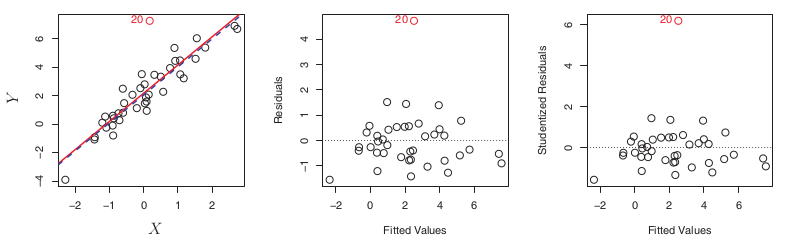
\includegraphics[width=\textwidth]{./chap/1chap/2sec/2images/2_9outliers.png}
	\end{center}
	\caption{Left:The least squared regression is shown in red
	and the least squared regression after removal outlier is
	shown in dashed blue line. Center: the residual plot identifies
	clearly the outlier value. Right: The studentized residual plot
	identifies outliers too}
	\label{fig:fig2.8}
\end{figure}



%\begin{lstlisting}
%numerics = ['int16', 'int32', 'int64', 'float16', 'float32',\
%'float64']
%num_df = df.select_dtypes(include=numerics).copy()
%outlier_limit = [[0, 0] for k in num_df.columns]
%percScore = outlier_limit.copy()
%
%for j,k in enumerate(num_df.columns):
%    n_bins = 30
%    bins = np.linspace(df[k].min(), df[k].max(), n_bins)
%    hist, edges = np.histogram(df.loc[:, k], bins=bins)
%    y = np.linspace(1, hist.max(, len(hist), dtype='int')
%    x = np.linspace(df[k].min(, df[k].max(, len(hist))
%    x_matrix, y_matrix = np.meshgrid(x, y)
%    mc = medcouple(df[k])
%    if mc > 0:
%        iq_adj = [1.5*np.exp(-4*mc), 1.5*np.exp(3*mc)]
%    else:
%        iq_adj = [1.5*np.exp(-3*mc), 1.5*np.exp(4*mc)]
%    low = np.percentile(df[k], 25) - iq_adj[0]*(np.percentile(df[k], 75) - np.percentile(df[k], 25))
%    up = np.percentile(df[k], 75) + iq_adj[1]*(np.percentile(df[k], 75) - np.percentile(df[k], 25))
%    outlier_limit[j][0], outlier_limit[j][1] = low, up
%    a, b = round(sci.percentileofscore(df[k], low), 2), round(sci.percentileofscore(df[k], up), 2)
%       					        
%    skew, kurt = round(sci.skew(df[k]), 1), round(sci.kurtosis(df[k]), 1)
%    fig, axs = plt.subplots(nrows=2, sharex=True)
%    fig.suptitle(f'Dot Plot (bins={n_bins}) and Box Plot,\
%        skew={skew}, kurtosis={kurt}')
%    axs[0].scatter(x_matrix, y_matrix, c=y_matrix<=hist, cmap='Greys')
%    axs[0].set_ylabel('Frequency Number')
%    axs[1].boxplot(df[k], flierprops=red_square, whis=(a, b), vert=False)
%    for ax in axs:
%        ax.set(xlabel=k)
%    outlier_limit_dict = {df.columns[j]:tuple(k) for j,k in enumerate(outlier_limit)}
%\end{lstlisting}

\begin{enumerate}
	\item \emph{M Estimation}
		It is an extension of the maximum likelihood estimate method, its priniciple is to
		minimize the residual funcion $\rho$:
		$\hat{\beta}_{M}=\min\limits_{\beta}\rho\left(y_{i}-\su{{j=0}}{p}x_{ij}\beta_{j}
		\right)$, we have to solve $\min\limits_{\beta}\su{{i=1}}{n}\rho(u_{i})=\min\limits_{\beta}\su{{i=1}}{n}\rho\left(\dfrac{y_{i}-\su{{j=0}}{p}
		x_{ij}\beta_{j}}{\sigma}\right)$.\\
		$\hat{\sigma}=\dfrac{MAD}{0.6745}=\dfrac{median\left(\epsilon_{i}-median(\epsilon_{i})\right)}{0.6745}$\\
		If we use Tukey's objective function we have
		$\rho$:
		$\begin{cases}
			\dfrac{u_{i}^{2}}{2} - \dfrac{u_{i}^{4}}{2c^{2}} + \dfrac{u_{i}^{6}}{6c^{4}},~
			|u_{i}| \leq c\\
			\dfrac{c^{2}}{6},~|u_{i}|>c
		\end{cases}$\\
		with $c=0.6745$
		We look for first partial derivative $\hat{\beta}_{M}$ to $\beta$ so that:\\
		$\su{{i=1}}{n}x_{ij}\psi\left(\dfrac{y_{i}-\su{{j=0}}{p}x_{ij}\beta}{\hat{\sigma}}
		\right)$ where $\psi=\rho'$. To solve this equation Draper and Smith have defined 
		a weighted function: 
		$\omega(\epsilon_{i})=
		\dfrac{\psi\left(\dfrac{y_{i}-\su{{j=1}}{p}x_{ij}\beta}{\hat{\sigma}}\right)}
		{\dfrac{y_{i}-\su{{j=1}}{p}x_{ij}\beta}{\hat{\sigma}}}$\\
		We can rewrite this equation with:
		$\omega_{i}=\begin{cases}
			\left[ 1-\left(\dfrac{u_{i}}{c}\right)^{2}\right]^{2},~|u_{i}| \leq c\\
			0,~|u_{i}| > c
		\end{cases}
		$
		We take $c=4.685$ for Tukey's bisquare weighted function, so the equation of partial
		derivatives becomes $\su{{i=1}}{n}x_{ij}\omega_{i}\left(y_{i}-\su{{j=1}}{p}x_{ij}
		\beta\right)=0$ that can be solved by Iterative Reweighted Least Squares (IRLS)
		In matrix notation $\bm{X}^{T}\bm{W}_{i}\bm{X}\beta = \bm{X}^{T}\bm{W}_{i}\bm{Y}$
		where $\bm{W}_{i}$ is a $n\times n$ matrix with its diagonal elements are the 
		weighted.

		\begin{enumerate}
			\item Estimate regression coefficients on the data using OLS
			\item Test assumptions of the regression model
			\item Detect the presence of outliers in the data.
			\item Calculate estimated $\hat{\beta}^{0}$ with OLS
			\item Calculate residual value $\epsilon_{i}=y_{i}-\hat{y}_{i}$
			\item Calculate value $\hat{\sigma}_{i}=1.4826\times MAD$
			\item Caluclate value $u_{i}=\dfrac{\epsilon_{i}}{\hat{\sigma_{i}}}$
			\item Calculate the weighted value $\omega_{i}$ 
			\item Calculate $\hat{\beta}_{M}$ using WLS with $\omega_{i}$
			\item Repeat steps (e)-(h) to obtain a convergent value of $\hat{\beta}_{M}$
			\item Test to determine whether independent variables have significant effect
				on the dependent variable
		\end{enumerate}
	\item S estimation
		Proposed by Rousseeuw and Yohai, it is based on residual scale of M estimation. The
		weakness of M estimation is the lack of consideration on the data distribution and
		not a function of the overall data because only using the median on as the weighted
		value. The S estimation method uses the residual standard deviation to overcome the 
		weakness of median.\\
		$\min\su{{i=1}}{n}\rho\left(\dfrac{y_{i}-\su{{j=1}}{p}x_{ij}\beta}{\hat{\sigma}_{s}}
		\right)$ with $\hat{\rho}_{s}=\sqrt{\dfrac{1}{nK}\su{{i=1}}{n}\omega_{i}e_{i}^{2}}$,
		$K=0.199$, $\omega_{i}=\omega_{\sigma}(u_{i})=\dfrac{\rho(u_{i})}{u_{i}^{2}}$
		and the initial estimate is $\hat{\sigma}_{s}=\dfrac{median\left(\epsilon_{i}-
		median(\epsilon_{i})\right)}{0.6745}$
		For IRLS weighted function $c= 1.547$
		\begin{enumerate}
			\item[(e)] Calculate residual value $\epsilon_{i}=y_{i}-\hat{y}_{i}$ 
			\item[(f)] Calculate value of $\hat{\sigma}_{i}=$
				\begin{align*}
				\begin{cases}
					\dfrac{median\left(\epsilon_{i}-median(\epsilon_{i})\right)}{
					\hat{\sigma}_{s}},& itertion=1\\
					\sqrt{\dfrac{1}{nK}\su{{i=1}}{n}\omega_{i}\epsilon_{i}^{2}},&
					iteration>1
				\end{cases}
				\end{align*}

			\item[(g)] Caluclate value $u_{i}=\dfrac{\epsilon_{i}}{\hat{\sigma_{i}}}$
			\item[(h)] Calculate the weighted value $\omega_{i}=$
				\begin{align*}
				\begin{cases}
					\begin{cases}
						\left[1-\left(\dfrac{u_{i}}{1.547}\right)^{2}
						\right]^{2},&|u_{i}|\leq 1.547\\
						0, &|u_{i}|>1.547
					\end{cases},&iteration = 1\\
					\dfrac{\rho(u_{i})}{u_{i}^{2}},&iteration>1
				\end{cases}
				\end{align*}
		\end{enumerate}
	


\end{enumerate}

We can also use a robust the M-Estimators for Robust Linear Modeling
\emph{M-Estimators} are a broad class of extremum estimators for which the objective function is
a sample average.\\
They are defined by: 
$\hat{\theta} = \min\limits_{\theta}\left(\su{{i=1}}{n}\rho(x_{i},\theta)\right)$
whith $\rho$ the objective function.
\begin{python}
model_robust = sm.RLM(y, X, M=sm.robust.norms.TukeyBiweight(c=4.685))
result_robust = model_robust.fit()
print(result_robust.summary())
print(model_robust.weights)
\end{python}


\subparagraph{High leverage points}
\tR{Outliers are points which have an unusual response $y_{i}$ for a 
given predictor $x_{i}$, whereas leverage points have a unusual value 
for $x_{i}$.}
\begin{figure}[H]
	\begin{center}
		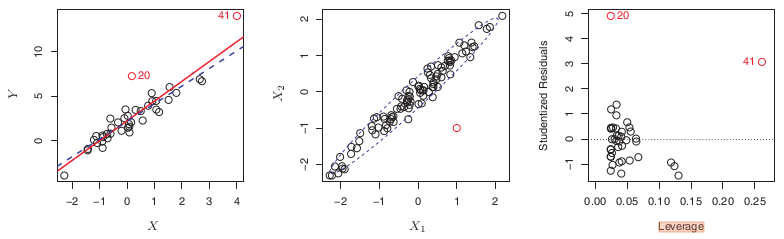
\includegraphics[width=\textwidth]{./chap/1chap/2sec/2images/2_10highLeveragePoints.png}
	\end{center}
	\caption{Left:Observation $41$ is a high leverage point, while
	20 is not.The red line is the least squared fit to all data,
	and the blue line is the fit with observation $41$ removed.\\
	Center:The red observation is not unusual in term of its $X_{1}
	$or its $X_{f2}$ value.\\Right: Observation $41$ has a high
	leverage and a high residual.}
	\label{fig:fig2.8}
\end{figure}
In simple linear regression is fairly easy to identify, since we can
simply look for observations for which predictors are outside of the
normal range of value of the observations.\\But in multiple linear
regression it is possible to have an observation that is well within
the range of each individual predictor's values (example graphic in the
middle). \sB{For data set with more than 2 predictors, it is difficult
to observe high leverage points, so we compute the} \emph{\tR{leverage 
statistic}}
\begin{center}
	\enc{$h_{i}=\dfrac{1}{n}+\dfrac{\left(x_{i}-\overline{x}
	\right)^{2}}{\su{{k=1}}{n}\left(x_{k}-\overline{x}
	\right)^{2}}$}\\
	\tR{A high $h_{i}$ value indicates a high leverage point.}
\end{center}
\begin{python}
results_ols = sm.OLS(y, X).fit()
sm.graphics.plot_leverage_resid2(results_ols)
plt.show()
\end{python}
To fix it Python does not contain an alternative at M-Estimator method (it is not robust against
leverage points), so we will use R functions

\emph{MM Estimation} aims to obtain estimates that have a high breakdown value and more efficient. 
Breakdown value is a common measure of the proportion of outliers that can be 
addressed before these observation affect the model.\\

\begin{enumerate}
	\item[(e)] Calculate residual value $\epsilon_{i}=y_{i}-\hat{y}_{i}$ 
	\item[(f)] Calculate value of $\hat{\sigma}_{i}=\hat{\sigma}_{s}$
	\item[(g)] Caluclate value $u_{i}=\dfrac{\epsilon_{i}}{\hat{\sigma_{i}}}$
	\item[(h)] Calculate the weighted value $\omega_{i}$ with $c=4,685$ as in
		M-estimation
\end{enumerate}

\emph{R code}
\begin{rcode}[deletekeywords={model, df}]
library(robustbase)

model_rob_mm <- lmrob(y ~ ., data=df) # MM-estimation
print(summary(model_rob_mm))
\end{rcode}
\subparagraph{Collinearity}
When there is a very highly correlation with each other we say that
they are \tR{collinear}. And this causes difficulties because to
separate out the individual effects.
\begin{figure}[H]
	\begin{center}
		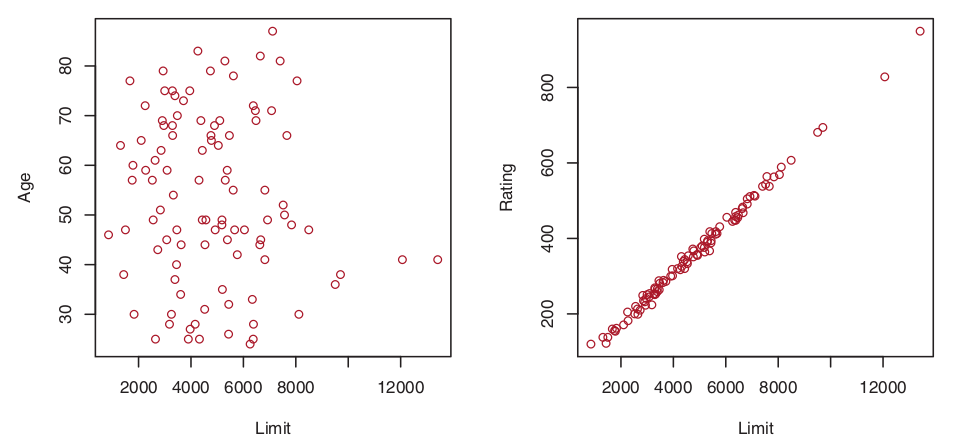
\includegraphics[width=\textwidth]{./chap/1chap/2sec/2images/2_11collinearity.png}
	\end{center}
	\caption{Scatter plot of the observation from credit data set.
	}
	\label{fig:fig2.8}
\end{figure}
\begin{figure}[H]
	\begin{center}
		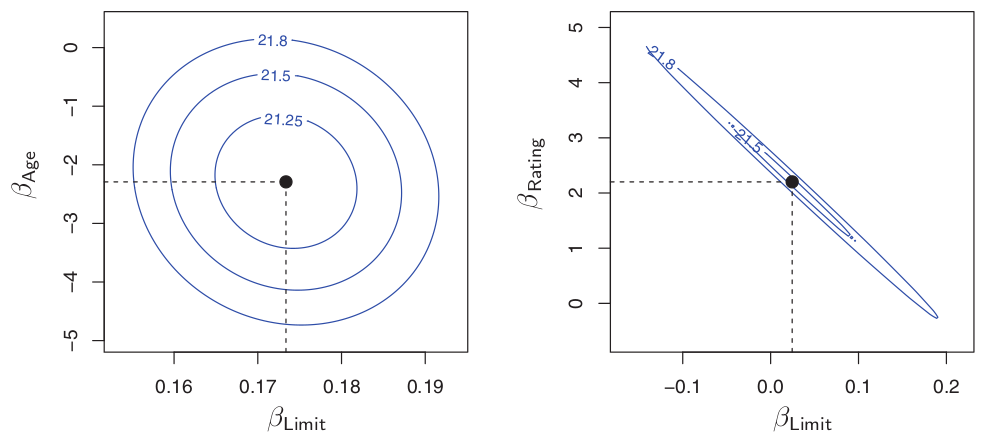
\includegraphics[width=\textwidth]{./chap/1chap/2sec/2images/2_12contourPlotCollinearity.png}
	\end{center}
	\caption{In each plot the black dot represents the coefficient
	values corresponding to the minimum value of RSS.\\
	Left: a contour plot of RSS for the regression of balance onto
	regression age and limit.\\Right:Because of the collinearity
	there are many pairs of $\beta_{Limit},\beta_{Rating}$ with a
	similar value of RSS.}
	\label{fig:fig2.8}
\end{figure}
\begin{figure}[H]
	\begin{center}
		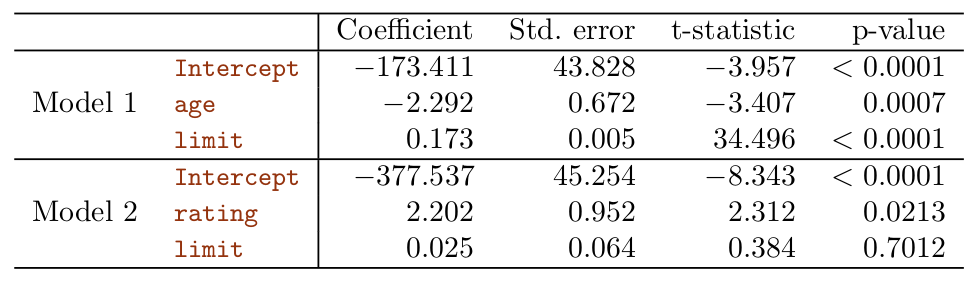
\includegraphics[width=\textwidth]{./chap/1chap/2sec/2images/2_13collinearModelAndNonCollinearModel.png}
	\end{center}
	\caption{Model 1 is a multiple regression of balance onto age
	and limit, then Model 2 is one of balance onto rating and limit
	\\The standard error of $\widehat{\beta}_{limit}$ increases
	12-fold in the second regression, due to collinearity.}
	\label{fig:fig2.8}
\end{figure}
Recall that for each predictor $\widehat{\beta}_{j}$ the associated
\emph{$t$-statistic} is divided by its standard error, consequently,
\tR{collinearity results in a decline in the \emph{$t$-statistic}}.\\A simple
way to identify collinearity is to observe the correlation matrix, but
if it exists collinearity between $3$ or more variables and no pair of
variables has a particularly high correlation we cannot detect 
collinearity, we call this \emph{multicollinearity}.\\Then a better way
to assess multicollinearity is to compute the \emph{\tR{variance 
inflation factor}} it is the ratio of the variance of $\widehat{
\beta}_{j}$ when fitting the full model divided by the variance of $
\widehat{\beta}_{j}$ if fit on its own. As a rule of thumb, \tB{a VIF
value that exceeds 5 or 10 indicates problematic amount of 
collinearity.}
\begin{center}
	\enc{$VIF\left(\widehat{\beta}_{j}\right)=\dfrac{1}{1-
	R_{X_{j}|X_{-j}}^{2}}$}\\
	\tB{$R_{X_{j}|X_{-j}}^{2}$ is the $R^{2}$ from regression of
	$X_{j} $ onto all of the other predictors.}
\end{center}
\begin{python}
import statsmodels.stats
from statsmodels.stats.outliers_influence import variance_inflation_factor as vif
print(pd.DataFrame({ 
  'VIF': [vif(X.values, i) for i in range(X.shape[1])],
  'index': X.columns}))
\end{python}

\subsection{ANOVA \& ANCOVA}
\paragraph{ANOVA}
%\subparagraph{Predictors with only 2 levels}
%One way of formulating the common-slope model is :
%$$ Y_{i} = \alpha + \beta X_{i} + \gamma D_{i} + \epsilon_{i}$$ where $D$, called a dummy-variable
%regressor or indicator variable, $$D1=
%\begin{cases}
%	1\text{ for women}\\
%	0\text{ for men}
%\end{cases}
%$$
%\begin{figure}[H]
%	\begin{center}
%		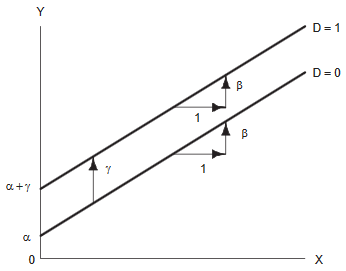
\includegraphics[width=.3\textwidth]{./chap/1chap/2sec/3images/1_graphicalDummy.PNG}
%	\end{center}
%	\caption{The parameters in the additive dummy-regression model}
%	\label{fig:1_graphicalDummy}
%\end{figure}
%
%\emph{gender} is a qualitative explanatory variable, with categories \emph{male} and \emph{female}
%the dummy variable $D$ is a regressor representing the explanatory variable gender.
%\subparagraph{Modelling interactions}
%$$ Y_{i} = \alpha + \beta X_{i} + \gamma D_{i} + \delta X_{i}D_{i} + \epsilon_{i}$$
%
%\begin{figure}[H]
%	\begin{center}
%		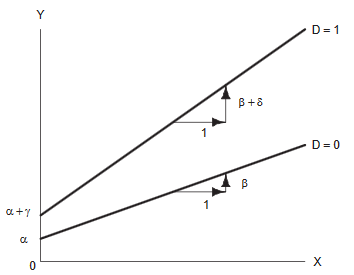
\includegraphics[width=.3\textwidth]{./chap/1chap/2sec/3images/2_graphicDummyInteract.PNG}
%	\end{center}
%	\caption{The parameters in the dummy-regression model with interaction}
%	\label{fig:1_graphicalDummy}
%\end{figure}

\subparagraph{ANOVA models}
Analysis of Variance describes \sB{the partition of the response variable sum of squares in a 
linear model into ``explained'' and ``unexplained'' components.}\\
\begin{itemize}
	\item Single categorical explanatory variable corresponds to One-Way ANOVA
	\item 2 factors to Two-Way ANOVA
	\item 3 factors to Three-Way ANOVA
\end{itemize}

\subparagraph{\emph{One-way} ANOVA}
\tR{examines equality of population means for a quantitative outcome and a 
single categorical explanatory variable with any number of levels}.\\
The term \tB{``one-way'' indicates that there is a single explanatory variable (``treatment'') 
with 2 or more levels and only one level of treatment is applied at any time for a given subject}.
\\
The term ``analysis of variance'' is a bit of misnomer, \tB{we use variance-like quantities to
study the equality or non-equality of population means}, so we are analyzing means, not variances.

\begin{center}
	The statistical model for which one-way ANOVA is appropriate is that the
	\begin{itemize}
		\item (Quantitative) Outcomes for each group are normally distributed
		\item Outcome variances are all equal to  ($\sigma^{2}$)
		\item The errors are assumed to be independent.
	\end{itemize}
\end{center}

\begin{center}
	\enc{$H_{0}:\forall (i,j) \in \inter{1}{k}^{2} \mu_{i} = \mu_{j}$}
\end{center}

In ANOVA \sB{we work with variances and also ``variance-like quantities'' which are not really the
variance of anything}, but are still calculated as $\frac{SS}{df}$ all of these quantities are
called ``mean squares''.\\

The deviation for subject $j$ of group $i$ in the figure above is mathematically equal to $Y_{ij}-
\overline{Y}_{i}$ where $Y_{ij}$ is the observed value for subject $j$ of group $i$ and $\overline{Y}_{i}$ is the sample mean for group $i$.
\begin{figure}[H]
	\begin{center}
		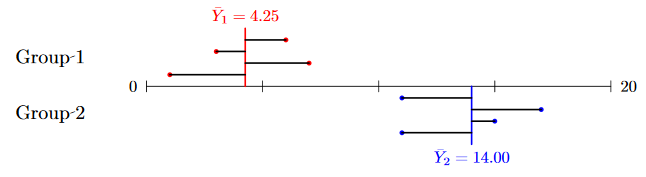
\includegraphics[width=\textwidth]{./chap/1chap/2sec/3images/3_anovaInterGrp.PNG}
	\end{center}
	\caption{Deviations for within-group of squares}
	\label{fig:3_anovaInterGrp}
\end{figure}
\begin{center}
\enc{
$ MS_{within} = \dfrac{SS_{within}}{df_{within}}
\begin{cases}
	SS_{within} = \su{{j=1}}{k}SS_{j}=\su{{j=1}}{k}\su{{i=1}}{n_{j}}\left(Y_{ij}-\overline{Y}_{\bullet j}
	\right)\\
	df_{within} = df_{j} = \su{{j=1}}{k}(n_{j}-1) = N-k
\end{cases}
$
}\end{center}

\tB{$MS_{within}$ is a good estimate of $\sigma^{2}$ from our model regardless of the truth of 
$H_{0}$.} This is due to the way $SS_{within}$ is defined.

\begin{figure}[H]
	\begin{center}
		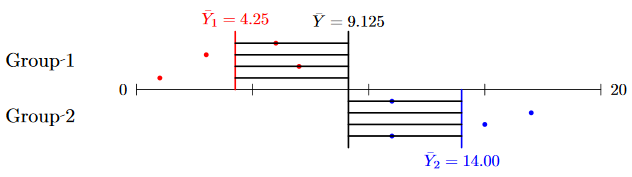
\includegraphics[width=\textwidth]{./chap/1chap/2sec/3images/4_anovaBtw.PNG}
	\end{center}
	\caption{Deviations for betwwen-group sum of squares}
	\label{fig:4_anovaBtw}
\end{figure}
$SS_{between}$ is the sum of the $N$ squared between-group deviations, where the deviation is
the same for all subjects in the same group. The formula is : 
\begin{center}
\enc{
$
MS_{Between} = \dfrac{SS_{Between}}{df_{between}}
\begin{cases}
SS_{between} = \su{{j=1}}{k}n_{j}\left(\overline{Y}_{\bullet j}-\overline{Y}\right)^{2}\\
df_{between} = k-1
\end{cases}
$
}\end{center}
Because of the way $SS_{between}$ is defined, \tB{$MS_{between}$ is a good estimate of $\sigma^{2}
$ only if $H_{0}$ is true}. Otherwise it tends to be larger. \\
The $F-statistic$ defined by $F=\dfrac{MS_{between}}{MS_{within}}$ \sR{tends to be larger if the
alternative hypothesis is true than if the null hypothesis is true}.\\

We can quantify ``large'' for the \emph{F-statistic}, by comparing it to its null sampling 
distribution which is the specific \emph{F-distribution}  which has degrees of freedom matching
the numerator and denominator of the \emph{F-statistic}.\\
Concerning inferences to build the confidence interval we need the \tB{\emph{standard error} (the
standard deviation of the means) that is $\sqrt{\dfrac{MS_{within}}{n_{i}}}$}\\

Numerically we have:\\
Given 2 samples with means $\mu_{1}$ and $\mu_{2}$, same variance $\sigma^{2}$ and $n=n_{1}+n_{2}$
observations.
Model: 
\begin{center}
	$\forall (j,i)\in\inter{1}{2}\times\inter{1}{n_{j}}y_{ij} = \mu_{i} + \epsilon_{ij} = \mu + \alpha_{j} + \epsilon_{ij}$
\end{center}
$\alpha_{j}=\mu_{j}-\mu$ is called (treatment-) effect

Decomposition:
\begin{align*}
	SS_{total} =& \su{{j=1}}{n_{1}}\left(y_{1j}-\overline{y}\right)^{2} +
	\su{{j=1}}{n_{2}}\left(y_{2j}-\overline{y}\right)^{2}\\
	=& \su{{j=1}}{n_{1}}\left(y_{1j}-\overline{y_{1}}+\overline{y_{1}}-\overline{y}\right)^{2}
	+ \su{{j=1}}{n_{2}}\left(y_{2j}-\overline{y_{2}}+\overline{y_{2}}-\overline{y}\right)^{2}\\
	=& \underbrace{(n_{1}-1)s_{1}^{2} + (n_{2}-1)s_{2}^{2}}_{SS_{within}} +
	\underbrace{n_{1}(\overline{y}_{1}-\overline{y}) + 
	n_{2}(\overline{y}_{2})-\overline{y}^{2}}_{SS_{between}}
\end{align*}
$SS_{between}$ corresponds to squared enumerator $(\overline{y}_{1} - \overline{y}_{2})^{2}$ of
the statistic: 
\begin{align*}
	SS_{between} =& n_{1}(\overline{y}_{1}-\overline{y})^{2} + 
	n_{2}(\overline{y}_{2}-\overline{y})^{2}\\
	=& n_{1}\left(\overline{y}_{1}-\dfrac{n_{1}\overline{y}_{1}+n_{2}\overline{y}_{2}}{n_{1}+
	n_{2}}\right)^{2} + n_{2}\left(\overline{y}_{2}-\dfrac{n_{1}\overline{y}_{1}+n_{2}
	\overline{y}_{2}}{n_{1}+ n_{2}}\right)^{2}\\
	=& \dfrac{n_{1}n_{2}}{n_{1}+n_{2}}\left(\overline{y}_{1}-\overline{y}_{2}\right)^{2}
\end{align*}
$SS_{within}$ corresponds to denominator of \emph{t-statistic}:
$s=\sqrt{\dfrac{(n_{1}-1)s_{1}^{2}+(n_{2}-1)s_{2}^{2}}{n_{1}+n_{2}-2}}$\\
Pooled variance that is an estimate of the fixed common variance $\sigma^{2}$ underlying various
populations that have different means.
$\hat{\sigma}=\dfrac{(n_{1}-1)s_{1}^{2}+(n_{2}-1)s_{2}^{2}}{(n_{1}-1)+(n_{2}-1)}$
Null hypothesis $H_{0}:\mu_{1}=\mu_{2}$ or $\alpha_{1}=\alpha_{2}=0$
\emph{F-test}
$\left(\overline{Y}_{1}-\overline{Y}_{2}\right)\hookrightarrow \mathcal{N}\left(\mu_{1}-\mu_{2},
\left(\frac{1}{n_{1}}+\frac{1}{n_{2}}\right)\sigma^{2}\right)\\
\E{\left[\overline{Y}_{1}-\overline{Y}_{2}\right]^{2}}=\left(\frac{1}{n_{1}}+\frac{1}{n_{2}}
\right)\sigma^{2}+(\mu_{1}-\mu_{2})^{2}\\
\E{MS_{between}}=\E{\frac{n_{1}n_{2}}{n_{1}+n_{2}}\left[\overline{Y}_{1}-\overline{Y}_{2}
\right]^{2}} = \sigma^{2}+\frac{n_{1}n_{2}}{n_{1}+n_{2}}(\mu_{1}-\mu_{2})^{2}\\
\E{MS_{whithin}}=\sigma^{2}\\
F = \dfrac{MS_{between}}{MS_{within}}$
Here $F=t^{2}$\\
\begin{align*}
	\text{Degrees of freedom} =& n - 1\\
	=& \underbrace{(n-m)}_{df_{within}} + \underbrace{(m-1)}_{df_{between}}
\end{align*}
\begin{itemize}
	\item $SS_{within}$ and $SS_{between}$ are independent
	\item under $H_{0}$ $\E{MS_{between}} = \E{MS_{within}} = \sigma^{2}$
	\item under $H_{a}$ $\E{MS_{between}}>\sigma^{2}$ and $\E{MS_{within}} = \sigma^{2}$
\end{itemize}
Hence $$ F= \dfrac{MS_{between}}{MS_{within}}\hookrightarrow F_{m-1,n-m}$$
In the case of 2 groups (``\emph{t-test}'') we received:
$$ \overline{y}_{1}-\overline{y}_{2} \pm t_{n-2,1-\frac{\alpha}{2}}s\sqrt{\frac{1}{n_{1}}+
\frac{1}{n_{2}}}$$
\subparagraph{Two-way-ANOVA}
If a quantitative explanatory variable is also included, that variable is usually called a 
\emph{covariate}.\\
The usual assumptions of normality, equal variance and independent errors apply.\\

\tB{ANOVA decomposes the total variance} present in the data into contribution of the single 
sources of variation :
\begin{itemize}
	\item \tB{systematic contribution}: differences of means
	\item \tB{random rest}: variability around group mean
\end{itemize}
We have the total variance law:
\begin{center}
\enc{
$
\begin{cases}
X\& Y\text{ random variables on the same probability space}\\
\text{variance of }Y\text{ is finite}
\end{cases}\Rightarrow
\V{Y} = \E{\mathbb{V}\left(Y|X\right)} + \V{\mathbb{E}\left(Y|X\right)}
$}
\end{center}

Numerically:
$$\forall (i,j,k)\in\inter{1}{m_{1}}\times\inter{1}{m_{2}}\times\inter{1}{n_{ij}}~y_{ijk} =
\mu_{ij} +\epsilon_{ijk},~\epsilon_{ijk}\hookrightarrow \mathcal{N}(0,\sigma^{2})$$
Decomposition of means:
\begin{align*}
	\mu_{ij} &= \mu + (\mu_{i}-\mu) + (\mu_{j}-\mu) + (\mu_{ij}-\mu_{j}-\mu_{i}+\mu)\\
	&= \mu +\alpha_{i} +\beta_{j} + \gamma_{ij}\\
	&= \text{``overall mean''} + \text{``main effect of A''} + \text{``main effect of B''} +
	\text{``interaction of A and B''}
\end{align*}
Null hypothesis:
\begin{itemize}
	\item All $\alpha_{i}=0$
	\item All $\beta_{j}=0$
	\item All $\gamma_{ij}=0$
\end{itemize}

\begin{python}
import statsmodels.api as sm

data = pd.read_csv('myFile.csv', sep=',')
model = sm.ols('y ~ C(X1, Sum)*C(X2, Sum)', data=data).fit()
table = sm.stats.anova_lm(model, typ=2) # typ=2 indicates that we are testing for each main effect
# after the other main effect.
print(table)
\end{python}

\paragraph{ANCOVA} The multiple regression model below would be equal to an ANCOVA, if \sB{$X_{1}$ was binary and $X_{2}$ was some covariate of interest}:$y = \beta_{0}+\beta_{1}X_{1}+\beta_{2}X_{2}+\epsilon$\\ The key is in the interpretation of the intercept value and the slope for the binary predictor.  If $X_{1}$ is binary with values 0 and 1, then the \begin{itemize} \item \textbf{\emph{intercept}} is the average of \tB{$\beta_{0}=\E{y|(X_{1},X_{2})=(0,0)} $} \item \textbf{\emph{slope}} represents the mean difference between 0 and 1 group\\ \tB{$\beta_{1} = \E{y|(X_{1},X_{2})=(1, x_{2})}-\E{y|(X_{1},X_{2})=(0, x_{2})}$}
\end{itemize}

\subparagraph{When is ANCOVA used?}
It is usually used for analysis of quasi-experimental studies, when the regression groups are
not randomly assigned and the researcher wishes to statically ``equate'' groups on one or more
variables which may differ across groups. 
\subparagraph{Relation to Repeated Measures ANOVA}
The repeated measures ANOVA (and the paired t-test) is equivalent to test if the average 
difference score is different from zero. However ANCOVA and Repeated Measures ANOVA tests are not
equivalent, because they represent 2 different ways of conceptualizing change.
\subparagraph{Adjusted Means} 
ANCOVA procedures will produce adjusted means, which represents the means of each group once the
covariate(s) has been controlled.\\ In Regression terms, these adjusted means come from the 
intercept: $\beta_{0}=\overline{y}-\beta_{1}\overline{X}_{1}-\beta_{2}\overline{X}_{2}$
\sB{Because the intercept represents the average value of $y$ when all predictors equal zero, we 
have to pay attention to the scaling of the variables.} If the grouping variable, $X_{1}$, has two
values 0 and 1, the adjustment leads to an intercept for the 0 group where the covariate, $X_{2}$,
is also equal zero. In many cases, the estimated mean when covariates are equal to zero is not
meaningful. So if using regression analysis and there is interest in obtaining the adjusted means,
\tB{it is common to rescale the covariates, $x_{2}=X_{2}-\overline{X}_{2}$}.\\
Then in regression analysis, the adjusted means can be computed by using the regression 
coefficients and inserting values for $X_{1}$\\ $\overline{Y}_{adj}=\beta_{0}+\beta_{1}X_{1}-\beta_{2}\overline{X}_{2}$

\subparagraph{Should I use ANCOVA or Regression?}
Test hypothesis about group differences using an ANCOVA procedure or a regression analysis will 
give the same result, when there are several categories for the independent variable or 
interactions are of interest we should use ANCOVA. 
\subparagraph{Sum of Squares}
The issue type  of sum of squares comes up in ANCOVA as it does in ANOVA: 

\begin{itemize}
	\item[Type \textbf{I}:] Each effect partials out or controls for only those effect
		entered before it. If effect $A$ is entered first, it does not partial out $B$ or 
		$A\times B$ added after it. But $B$ can partial out $A$, and interaction $A\times
		B$ partials out $A$ and $B$
	\item[Type \textbf{II}:] Each effect at the same step or before is controlled but not for
		later steps. Say $A$ and $B$ are entered first and then $A\times B$ is added. $A$
		controls for $B$ and $B$ controls for $A$. Neither controls for $A\times B$, but
		$A\times B$ controls for both $A$ and $B$.
	\item[Type \textbf{III}:] adjusts fro all other factors or variables in the model. 
\end{itemize}

\emph{R code}
\begin{rcode}[deletekeywords={model, df}]
model_ancova <- aov('y ~ f1 + f2*x1', data=df)
print(summary(model_ancova))
\end{rcode}


